\documentclass[10pt]{article}
%Have "Packages.tex" in a folder called "Includes"
%Have "SDU_logo.png" in a folder called "Figures"
%Have "Appendix0.tex" in a folder called "Appendix"
%Have "Bibliography.tex" in a folder called "Sections"

% Margin på 3cm både i top, 2,5 i venstre og 3,5 i højre
\usepackage[total={6.5in,8.75in},top=3cm, bottom=3cm, left=2.5cm, right=3.5cm, includefoot]{geometry}

\usepackage[utf8]{inputenc}

% Gør det muligt at sætte billeder ind
\usepackage{graphicx}

% Bruges til at lave subFigures
\usepackage{mwe}

\usepackage[export]{adjustbox}
\usepackage{float}

% Formler og græske symboler
\usepackage[euler]{textgreek}
\usepackage{amsmath}

% At \par flytter den rigtige længde
\usepackage{parskip}
    \setlength{\parskip}{1 em}

% 1,5 linjeafstand, skrifttypen New Century Schoolbook og ingen højre allignment
\renewcommand{\baselinestretch}{1.3}
\usepackage{newcent}
\usepackage[document]{ragged2e}


%Gør at referencer og navne på figurer og tabeller er på engelsk.
\usepackage[english]{babel}

% Links bliver blå, fx mails, og man kan klikke på det.
\usepackage{hyperref}
\hypersetup{
					colorlinks, 
					linkcolor={black},
					citecolor={black},
					urlcolor={blue}
					}
					
% Referenceliste
\usepackage[sorting=none]{biblatex}
\addbibresource{includes/references.bib}

%Gør at man kan få tekst til at gå rundt om billeder.
\usepackage{wrapfig}

%Giver mulighed for flere linjer i captions mm.
\usepackage{caption}

%Gør det muligt at få subfigures, flere forskellige billeder i en figur
\usepackage{subcaption}

%giver mulighed for at bruge \textdegree{}
\usepackage{textcomp}
%giver mulighed for \degree i mathmode
\usepackage{gensymb}
%sætter sidetal til x af y
\usepackage{lastpage}
\usepackage{fancyhdr}
\pagestyle{fancy} 
\cfoot{\thepage\ of \pageref{LastPage}}

%pakke til at lave tables
\usepackage{array}
    \newcolumntype{P}[1]{>{\centering\arraybackslash}p{#1}}

% giver mulighed for at lave C++ code snippets.
\usepackage{listings}
\usepackage{xcolor}
\definecolor{codegreen}{rgb}{0,0.6,0}
\definecolor{codegray}{rgb}{0.5,0.5,0.5}
\definecolor{codepurple}{rgb}{0.58,0,0.82}
\definecolor{backcolour}{rgb}{0.95,0.95,0.92}
\newcommand{\mc}[2]{\multicolumn{#1}{c}{#2}}
\definecolor{Gray}{gray}{0.85}
\definecolor{toprow}{rgb}{0.52, 0.52, 0.51}
\definecolor{emerald}{rgb}{0.31, 0.78, 0.47}
\definecolor{gold(web)(golden)}{rgb}{1.0, 0.84, 0.0}
\definecolor{persianred}{rgb}{0.8, 0.2, 0.2}
\definecolor{ao(english)}{rgb}{0.0, 0.5, 0.0}
\newcolumntype{a}{>{\columncolor{Gray}}c}
\newcolumntype{b}{>{\columncolor{white}}c}
\newcolumntype{?}[1]{!{\vrule width #1}}
\definecolor{Red}{rgb}{1,0,0}

%\definecolor{backcolour}{rgb}{0.67,0.74,0.73}
\lstdefinestyle{mystyle}{
    language=C++,
    backgroundcolor=\color{backcolour},
    commentstyle=\color{codegreen},
    keywordstyle=\color{magenta},
    numberstyle=\tiny\color{codegray},
    stringstyle=\color{codepurple},
    basicstyle=\ttfamily\footnotesize,
    breakatwhitespace=false,         
    breaklines=true,                 
    captionpos=b,                    
    keepspaces=true,                 
    numbers=left,                    
    numbersep=5pt,                  
    showspaces=false,                
    showstringspaces=false,
    showtabs=false,                  
    tabsize=2
}
\lstdefinestyle{base}{
  language=C,
  emptylines=1,
  breaklines=true,
  basicstyle=\ttfamily\color{black},
  moredelim=**[is][\color{red}]{@}{@},
}

\lstset{style=mystyle}

% Kan tilføje farver til tabeller
\usepackage{colortbl}
\usepackage{titlesec}
\setcounter{secnumdepth}{4}
\titleformat{\paragraph}
{\normalfont\normalsize\bfseries}{\theparagraph}{1em}{}
\titlespacing*{\paragraph}
{0pt}{3.25ex plus 1ex minus .2ex}{1.5ex plus .2ex}

%Kan bruges til at indsætte quotes.
\usepackage{csquotes}

%Centrerer titler i tabeller.
\usepackage{booktabs}

%bruges til at gøre alle kolonner samme størrelse
\usepackage{tabularx}

%For at få nummer på references afsnit
\usepackage[numbib]{tocbibind}

\usepackage{hhline}

%Changing space below figures
%\setlength{\belowcaptionskip}{-20}

\title{
%SDU Logo
    \vspace{-1 cm}
    
\includegraphics[width=50mm,right]{figures/SDU_logo.png}\\
    \vspace{1.5 cm} %Vertical space in between logo and title
    \textbf{Semesterproject}\large\\
     in Signals and Robot Systems\\
     \vspace{1 cm} %Vertical space to next table
  

%Space for inserting small picture if needed
\begin{figure}[H]
    \centering
    %\includegraphics[width = 9.5 cm]{figures/frontpage.png}
    \caption{Relevant caption}
    \label{fig:frontpage}
\end{figure}

\begin{table}[h] %Supervisor(s)
    \centering
    \thispagestyle{empty}
    \begin{tabular}{l l}
    Supervisor & Iñigo Iturrate \\
    Hand in date & 19. dec 2025 \\
    Institution & University of Southern Denmark\\
    Group & 1 \\
    
    Study Program & Diplomingeniør i Robotteknologi
    \end{tabular}
        \vspace{-1 em}
\end{table}

\vspace{0,25 cm}
 \noindent\rule{9.5 cm}{0.4pt}
\vspace{0,25 cm} %Vertical space between supervisor(s) and participants 

\begin{table}[h]
\vspace{1 em}
    \centering
    \begin{tabular}{l|l}
    Daniel Edsbjerg Holst Poulsen & \href{mailto: dpoul24@student.sdu.dk}{dpoul24@student.sdu.dk}  \\
    Dominik Felten & \href{mailto: dofel22@student.sdu.dk}{dofel22@student.sdu.dk} \\
    Frederik Svend Vester & \href{mailto: frves24@student.sdu.dk}{frves24@student.sdu.dk} \\
    Mads Riis Olsen & \href{mailto: madsr16@student.sdu.dk}{madsr16@student.sdu.dk} \\
    Magnus Hansen & \href{mailto: magnh24@student.sdu.dk}{magnh24@student.sdu.dk} \\
    Sebastian Aksornnarong Nielsen & \href{mailto: sebni24@student.sdu.dk}{sebni24@student.sdu.dk} \\
    \end{tabular}
            \vspace{-3 em}
\end{table}    
}\small
\date{}
\author{}
%End of front page setup

\begin{document}
\maketitle
\thispagestyle{empty}
\setcounter{tocdepth}{3} 
\newpage
%Abstract section
\begin{abstract}
    \label{sec:Abstract}

In this project, software has been developed to automate the process of picking up and throwing a ball using a "Universal robotics" (UR) arm
For the purpose of demonstrating a UR arm, combined with a camera can be utilized for performing coordinated actions.
the minimum acceptable threshold for success is picking up a ball with a pair of grippers, and throwing it at a defined target. 
Before doing so, the event needs to be simulated to validate the robot kinematics and throwing trajectory, before physically executing the action.
The software integrates object detection through a camera, a trajectory calculation and robot control into a single framework.

The software is compatible with a "Universal Robots - UR5" robot arm, combined with a "WEISS ROBOTICS" GCL GRipper and
a camera "Basler acA 1440-220uc". The software is written in C++ with usage from a large variraty of libraries, compiled on a personal computer.
The trajectory calculation and robot kinematics for the throw is done through "Matlab", the camera vision detection depends on the library "OpenCV", 
the robotics control is largly dependend on the library "UR RTDE" and the simulation is also created through "Matlab".
Other items for the project, such as the ball and basket has been made using CAD tools and 3D printed in PLA material.
The softare acts as hub for combining all the different factors, giving full coordination and overview on the different components for a functional robotic throwing system.
\end{abstract}

\newpage
\thispagestyle{empty}
\tableofcontents
\thispagestyle{empty}
\newpage
%\setcounter{page}{1}


%Sections

% Indsæt sider med nedenstående format:
%\section{$TITLE$}
%\input{sections\$YOUR_PAGE$}

\section{Introduction} 
\input{sections/Introduction.tex}
\newpage

\section{System Overview} 
\input{sections/SystemOverview.tex}
\newpage

\section{Robot Calibration} 
The table-robot calibration was done according to the provided protocol \cite{calibrationProtocol}. All the calculations were done in MATLAB \cite{matlab2024b} using the Robotics Systems Toolbox \cite{roboticsToolbox} and the script is included in the appendix. The placement of the world frame can be seen in figure~\ref{fig:worldFrame}. 

\begin{figure}[H]
  \centering
  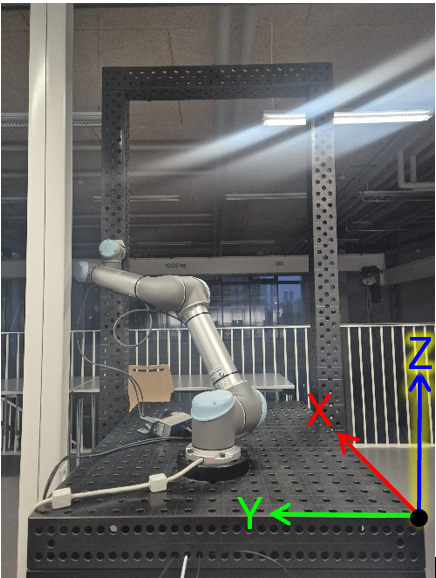
\includegraphics[width=0.5\textwidth]{figures/Worldframe1.png}
  \caption{Placement of the world frame.}
  \label{fig:worldFrame}
\end{figure}

 
Overall, 72 points were measured in both the world frame and robot base frame, and the data is included in the appendix. Of these 72 points, every third point was used for the testing set and the remaining 48 points were used for the training set. The size of the testing set was therefore 24. The calculated world to base transformation is shown below (\ref{eq:world_to_base}). 

\begin{equation}
\label{eq:world_to_base}
\text{world\_to\_base} =
\begin{bmatrix}
0.3841 & -0.9233 & 0.0004 & 0.2743 \\
0.9233 &  0.3841 & -0.0011 & 0.4247 \\
0.0009 &  0.0008 &  1.0000 & 0.0347 \\
0      &  0      &  0      & 1.0000
\end{bmatrix}
\end{equation}

And the corresponding base to world transformation is shown below (\ref{eq:base_to_world}).

\begin{equation}
\label{eq:base_to_world}
\text{base\_to\_world} =
\begin{bmatrix}
0.3841 &  0.9233 &  0.0009 & -0.4975 \\
-0.9233 & 0.3841 &  0.0008 &  0.0902 \\
0.0004 & -0.0011 &  1.0000 & -0.0343 \\
0      &  0      &  0      &  1.0000
\end{bmatrix}
\end{equation}

As the URDF files require the rotational part of the transformation to be provided as “roll pitch yawn” this was also calculated for the world to base transformation. The result is shown below (\ref{eq:rollPitchYawn}).

\begin{equation}
\label{eq:rollPitchYawn}
\text{rollPitchYawn} =
\begin{bmatrix}
0.0008 & -0.0009 & 1.1766
\end{bmatrix}
\end{equation}
 
The base to world transformation was then tested on the 24 points of the testing set to calculate the root mean square error \cite{rmsDeviation} which is shown in the table below (table~\ref{tab:rmsError}). Additionally, the error for each axis in the world frame was also calculated, which is highest in the x-direction and lowest in the z-direction (table~\ref{tab:rmsError}).

\begin{table}[H]
  \centering
  \caption{Overall and per axis root mean square error (mm) \cite{rmsDeviation} for the table-robot calibration.}
  \label{tab:rmsError}
  \begin{tabular}{|l|c|}
    \hline
    Axis in the world frame & Root mean square error (mm) \cite{rmsDeviation} \\ \hline
    Overall & 0.20872 \\
    X-axis  & 0.26483 \\
    Y-axis  & 0.20528 \\
    Z-axis  & 0.13569 \\ \hline
  \end{tabular}
\end{table}

Moreover, a heat map of the x-y plane of the world frame was generated to show local differences for the error. The heat map shows that the local error varies between 0.10 mm and 0.55 mm. The highest local error is for high x-values and low y-values (figure~\ref{fig:heatMap}).

\begin{figure}[H]
  \centering
  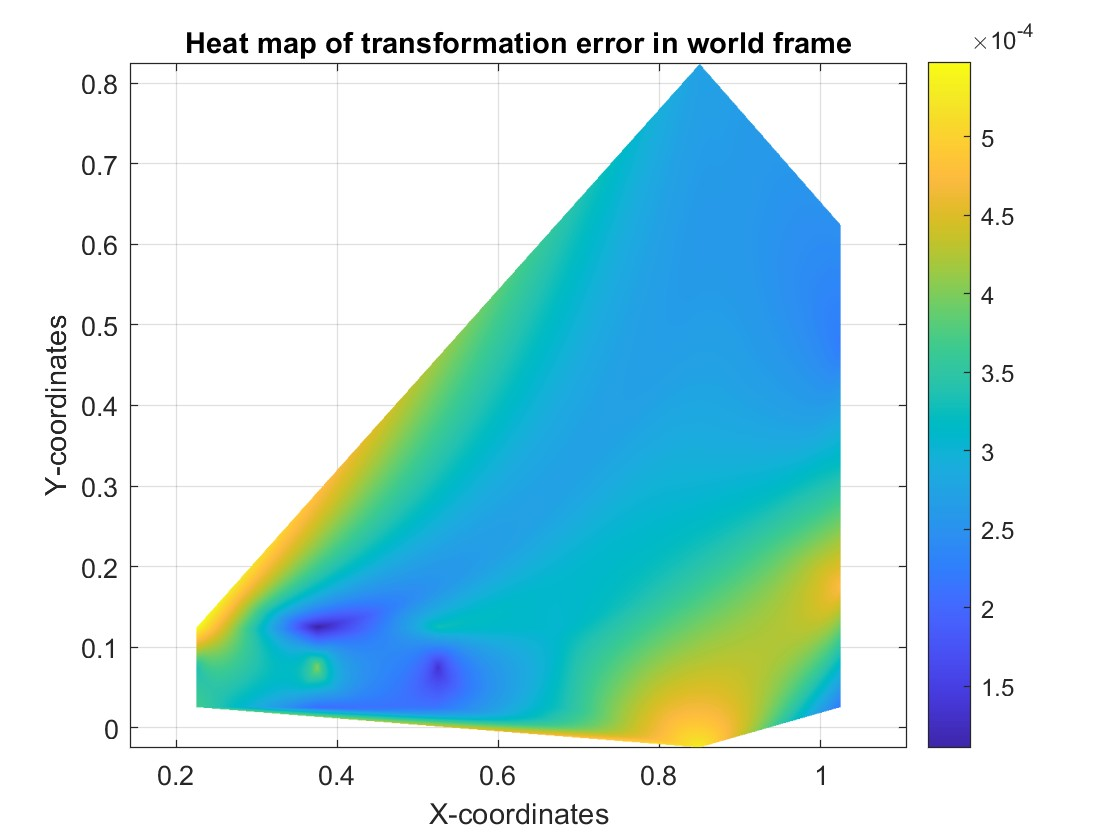
\includegraphics[width=0.7\textwidth]{figures/heatmap_new.jpg}
  \caption{Heatmap of the local calibration error (mm) mapped over the x-y-plane in the world frame.}
  \label{fig:heatMap}
\end{figure}
 
Finally, the errors for different sample sizes of the training set were calculated. The graph shows that the error decreases with increasing sample sizes between sample sizes of 4 and 22 and then stays roughly the same from there until the maximum sample size of 48 (figure~\ref{fig:sampleSizes}).

\begin{figure}[H]
  \centering
  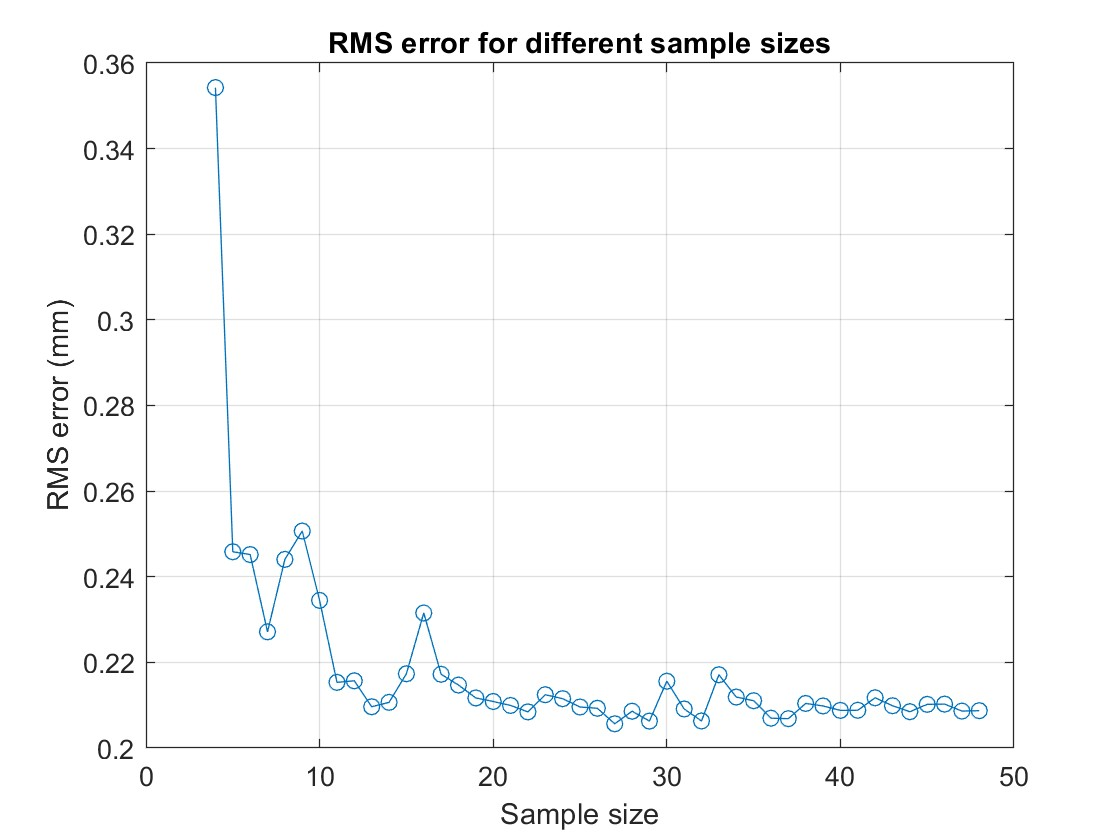
\includegraphics[width=0.7\textwidth]{figures/samplesizes_new.jpg}
  \caption{Root mean square error (mm) for different sample sizes from 4 to 48. The same testing set of 24 points was used on the base to world transformations calculated for each subset of training points.}
  \label{fig:sampleSizes}
\end{figure}

\newpage

\section{Controlling the Robot \& Gripper} 
 \label{sec:RobotControl}

Being able to control and move our robot and gripper is imperative to the success of our project as our goal of throwing an object relies on our ability to pick said object up and move it in a desired path.
\subsection{Gripper Control}
Our supplied gripper, the Weiss Robotics WSG50, allows us to pick up and throw our ball by enclosing it's fingers and opening them up again when appropriate.
To connect to the gripper, we set up a tcp connection to the grippers IP and port which allows us to send it commands.
We use these commands to open and close our gripper when appropriate at a speed of 420 mm/s which is the maximum speed the gripper can operate at.
%skrive om TCP kommunikation og hvordan vi får svar fra gripperen måske nævn testen hurtigt

\subsection{Robot Control}
Using the library UR\_RTDE, we are able to connect to and control our UR5 robot directly from our program.
This library allows us to send commands to the robot in real time without having to make our own URscript code.

The two classes we mainly use from this library is the RTDEControlInterface and RTDEReceiveInterface classes.
The RTDEControlInterface class allows us to send commands to the robot such as moving it to a specific position and setting its speed.

There are several motion types for our robot and different situations where it is appropriate to use each.
\begin{itemize}
    \item MoveL
    \linebreak- Used to move in straight cartesian paths which could be useful for picking up our ball initially as it could prevent unnecessary collisions with our ball or environment.
    \item MoveJ
    \linebreak- MoveJ moves the robot through joint-space allowing the robot to reach it's position in the most efficient manner possible. Could be used to move the robot in a throwing motion.
    \item ServoJ
    \linebreak- ServoJ, like moveJ, moves linearly in joint-space. ServoJ however allows us better control over the robot's trajectory as it is better suited for continous smaller movement like we would receive from our MATLAB script. ServoJ will not stop or slow down until it stops receiving new commands which is why it is better suited for our throwing motion.
\end{itemize}
The RTDEReceiveInterface class allows us to receive data from the robot such as its current position both in joint space and cartesian space which we mainly use for troubleshooting.


Using the function, setTargetPayload we are also able to alter the payload of the robot to offset the added weight of the ball, however since the ball weighs so little, the difference would be negligible and we therefore decided not to implement this. %måske skriv om hvad det betyder for robottens bevægelse
\subsection{Implementation}
Picking up the ball requires a combination of moving both the robot and gripper.
\subsubsection{Picking up the ball}
First, we receive the position of the ball in world coordinates from the vision system as well as the location of our container. %skal måske uddybes mere hvis det ikke er i vision delen
%these coordinates are then converted to a $4\times4$ transformation matrix based on our calibrated frame and is then flipped around the Y-axis to ensure the tool is facing downwards.
To avoid collisions, the robot first moves to a position directly above the detected ball using a fixed height.
Once above the ball, a command is sent to the gripper to open its fingers at the predefined speed.
The robot then moves directly down to the ball's position using moveL function which ensures a straight line movement in cartesian space.
Another command is sent to the gripper to close its fingers to pick up the ball and return to it's previous position using moveL.

\subsubsection{throwBall}
To throw the ball, the function only requires the coordinates it should throw to. It takes base coordinates and transfer them to world coordinates, because when we started developing, all was in the robots perspektive. So everything began in base coordinates.
The function will delete one of the files we use to transfer vectors, from matlab to c++(timeVector.txt). This is to make sure we do not repeat an old move, if the new one should fail.
The time it takes to run the matlab script is really annoying, but it is what happens next. It is only then we can throw the ball, so that means we are up for quite a delay.

To make sure we can get the highest priority on all systems, we have choosen to the actually throw in a thread. So if the matlab script run successfully, we will launch a qthread and give it highest priority, so we avoid any lag in the throw.
There is no special reason why we used Qthread over std::thread here with lambda. Either could have done it. 
It is a Qt class and it is properly the right reason to do use qThread over std::thread, but the real reason is more that it was cool to try like this with lambda instead of a function.

To do the throw, we are using two different commands:
\begin{itemize}
    \item moveInVectorPosWithRecoveryAndRelease(accelerationPositionsVector, deaccelerationsPositionsVector, timeStep)
    \linebreak- This function will use servoJ to move between iterations in q positions with steps in time given by timeStep. DeaccelerationsPositionsVector has been disabled due to throw being hard to measure if incorrect.
    \item moveInVectorSpeedWithRecoveryAndRelease(accelerationPositionsVector, accelerationSpeedVector, deaccelerationsSpeedVector, timeStep)
    \linebreak- This function will use speedJ to move between iterations in q speed with steps in time given by timeStep. DeaccelerationsPositionsVector has been disabled due to throw being hard to measure if incorrect.
    This function also uses the position to detect if it is off target and to try correcting the issue through the move.
\end{itemize}

We will show the test further down however to give a resume, speedJ gives us the most flowing motions, but is off target. - And throw is inconsistent. 
This is due to trajectories changing the course very rapidly and us overshooting a bit everytime and it building up. 
We have done some effort to get it on target by alternating the course a bit everytime it updates so it is consistent with the points given by the matlab script.

servoJ gives us the most precise motions, but is a bit laggy on the wrong computer... Throw is consistent.

With either commands timing of release is inconsistent. Sometimes it throws too early, sometimes too late, sometimes perfectly. - But totally inconsistent.

We hardcoded the release of the gripper, to throw 100 steps before the end of the vector. We always have a 126 steps vector on our throw when we use a 0.008 time step.
This is not the best way and should be a timevalue, but the inconsistent timing of the release made it useless no matter what we did and we finished the project here on the last day of the project.

We will write more about the difference in evaluation.




\newpage

\section{Camera Vision} 
\label{sec:camera}

In this project, an essential part of the problem was to find objects using a camera.
This was done using a Basler camera of the model acA 1440-220uc, which was outfitted with a C125-0418-5M lens.

To communicate with the camera, we used the Basler Pylon Camera Software Suite (Basler Pylon SDK).
This allowed us to interact with the settings stored in the camera, and get an image output.
This image was distorted, and we therefore needed to undistort it.
With an undistorted image, we could then find the coordinates of objects in the image.
For communicating points on the table, we defined world frame to span from a specific corner on the worktable.
Therefore, we also needed to make a homography to transform the coordinates in camera frame to world frame.
The coordinates of objects in the image could then be transformed into world frame, so they could be used by the rest of the program.

\subsection{Camera Calibration}
First, we needed a picture from the camera, which we can process and extract the necessary information from.
To achieve this, we first established a connection with the camera using "Pylon Viewer", a program included in the Basler Pylon SDK.
The Basler Pylon SDK also includes the library, which we utilised to control the camera directly from our program.
Using the pylon library, we were able to adjust the settings of the camera to make the image properly readable to a person. 

A computer program can in some applications, depending on its way of implementation, function partially or fully, even with an image not readable by humans.
This is because of the nature of image processing, as it relies on the data stored in the individual pixels.
The change from pixel to pixel is then analysed in different ways to pick up patterns and defining factors. 
The way we humans understand what we see, is done through pattern recognition, and rely less on the specific data of indivual "pixels".

Because of this, we had to test different configurations of the camera, so the image output would represent the real world as accurately as possible.
This was done through trial and error, and relied on human perception, so an element of human error is to be expected. 
This should not cause any major issues though, since the features of the image stays relative, and therefore are not changed through the camera configuration.
The output image could now be shown to the user, as part of our GUI, or for troubleshooting the output of our object detection. 

With the camera configured, we could then shift our focus to camera calibration.
This was done using the OpenCV library, which includes a number of functions, that simplify the undistortion and transformation of our images.
First, we took 30 pictures using the camera, where a chessboard is placed in different positions and orientations. 
Using OpenCV we can then find the inner corners of the chessboard, and their coordinates.
We also need the size of the squares and the number of inner corners on the chessboard, which are used to undistort the image.
Using these data, OpenCV is then able to calculate a list of vectors and matrices, which can then be turned into two maps.
These maps are offsets in the x and y direction, which we can then use to remap the distorted image, thereby undistorting it.

With the undistorted image, we now needed to make a homography, which could be used to transform coordinates between the camera frame and world frame.
To do this, we first made a simple homography using 4 coordinates in world frame, and the corresponding 4 coordinates in camera frame.
We then tested this homography by transforming a set of coordinates between camera frame and world frame.
These transformed coordinates were then compared to the corresponding coordinates, meassured directly in world frame.
This showed an offset of up to half a centimeter, depending on position in the image.
This offset may not fully ruin the functionality of the program by itself, but all the errors throughout the system can stack up, which is a major concern.
To ensure the best accuracy across the whole system, it is essential to reduce inaccuracies and calibration errors, wherever possible. 

As we had only used 4 sets of coordinates to make the homography, and got a suboptimal homography in return, we decided to extend and improve our dataset.
Instead of relying solely on human accuracy, we decided to add feature detection as part of the process.
This way, we were able to remove some of the human inaccuracies, and enabled us to extend our dataset considerably.
This was done by using the circle Hough transform, which made us able to find the holes located in the table. 
We assume that the holes are placed in a flat plane with a constant distance between them.
This is because the table shows signs of being cnc milled, which is a manufacturing process with relatively high accuracy, which we hope will be sufficient.

Using the circle Hough transform, we were able to determine the coordinates of the holes in the table.
We then set up a list of coordinates, resembling the real world coordinates of the holes.
The circle Hough transform returns more circle coordinates, than there are holes in the table, and we therefore needed to sort the output before use.
This was done using the first homography, which was calculated from 4 hand-picked coordinates.
Using this homography, we transformed the real world coordinates of the holes into the image frame.
With the world coordinates transformed into the image frame, we could then compare them to the image coordinates of the holes.
We then used the coordinates with the smallest offset to create a new homography.
This homography could then be used like the first one, while being more accurate to the plane.
Using these homographies recursively gives us a final homography with less human inaccuracy than the homography from human input.

During testing it was discovered, that there was an offset between the real world coordinates, and the coordinates returned, when converting from a point in the image to a point in world frame. 
By obtaining data from different areas of the table, we could deduce, that the offset increases as we travel away from a specific point.
Another important detail is, that this increase was growing, so as we moved away from the central point, not only did the offset increase, but it increased faster the further away the point was.
A linear function would therefore not be sufficient in correcting our coordinates.
Another idea for correcting these coordinates would be to meassure a set of data points with their world coordinates and the coordinates seen from our camera, and use these for interpolation.
We decided against interpolation, as the coordinates seen from the camera, could vary depending on what pixel the hough transform chose as the center point.
These small variations would have an imediate effect on the output coordinates, as interpolation only used the points around the desired coordinates.
At first we did not consider a different homography to allign our image coordinates with their relative world coordinates, so polynomial functions seemed like the best option.
We therefore decided to use polynomial functions, as we would then be able to encorporate all the data points and hopefully correct our coordinates.

To calculate the functions for converting our coordinates with offset into the correct world coordinates, we detected the ball in 64 places in a 8x8 grid of points with 10cm between the points in the x- and y-direction.
This data was then compared to the expected coordinates for each point, which was then used to create the fourth degree polynomial functions for the offset in the x- and y-direction. 
Originally we wanted to use second degree polynomials to convert the coordinates, but due to some issues when calculating the functions, the second degree polynomials created nonsensical results. 
Because of this, we decided to use the fourth degree polynomial, which did not cause issues, and therefore integrated it into the program.
Only later, when we had decided to stop development, was the issue resolved, so a second degree polynomial could be calculated.
We decided to stay with the fourth degree polynomial anyways, as this was the one used during testing, and therefore the one with the most data backing its validity.


\subsection{Object Detection}
Our object detection is split into two parts.
One part is to find the coordinates of the throwable object, in this case our 3D-printed ball.
The other part is for finding the middle of the target box, which we have also 3D-printed.

\subsubsection{Finding throwable object}
When the first iteration of our object detection was created, only the throwable object was meant to be found with machine vision. 
This was early on in the semester, where we were only introduced to specific tools through the "Machine Vision" course.
Having limited knowledge about the OpenCV library, and its extensive capabilities, we created the first iteration of our object detection with a simple form of threshholding, and later found connected pixels.
This was done by converting the image to HSV, which is more intuitive to people, and then choosing threshholds that seperate our throwable object from the background, creating a binary image.
All connected pixels of either 1 or 0 are then given the same nubmer as all the pixels they are connected to, which posess the same binary value.
This effectively creates individual objects, which fill up a specific area in the image. 
By then taking the average x- and y-values of each objects, we found the centers of the objects.

The issue with this approach is, that if two objects touch each other,their binary "shadow" will merge and contain all the area between the two objects, therefore outputting the center of the merged object.
Luckily we were later introduced to the Hough transform, which is a way to find simple features in an image.
By using the Hough circle transform, we were able to find our objects while avoiding the merging of objects.
The coordinates can from here be transformed from image coordinates into the desired coordinates format, which can then be passed on to the rest of the program.

\subsubsection{Finding target}
The task of finding the target box, was done by going back to the first idea used, when we started making the object detection. 
Our target is square, so the Hough circle transform was out of the question, and the Hough transform for lines could be tricky to apply, as most objects in the image already consist of lines.
Therefore we ended up converting the image to HSV, finding threshholds manually, and labelling the different objects.
Afterwards we could then find the centers of the objects, and output the coordiantes in a vector, in case multiple targets were in use. 
\newpage

\section{Projectile Trajectory} 
The calculation of the projectile trajectory is being done in MATLAB \cite{matlab2024b}. To do that all the target coordinates in the world frame, the radius of the projectile and the mass of the projectile were written to a text file which then is read by the MATLAB \cite{matlab2024b} script. The radius and mass of the projectile were defined in the main program and not hardcoded into the MATLAB \cite{matlab2024b} script to easier allow for the implementation of logic to choose between different projectiles later. The drag coefficient for a sphere \cite{dragCoefficient}, the air density \cite{airDensity} and gravitational acceleration vector \cite{gravity} were directly defined in MATLAB \cite{matlab2024b}. The release position vector was defined dynamically, depending on the target coordinates. This was done to find suitable inverse kinematic solutions within the specified joint limits for a wider range of target points (see table 2,3 section kinematic solutions). To simulate the trajectory between the release point and the target point an ordinary differential equation for the flight curve of the projectile was solved numerically with “ode45” \cite{ode45} for a specified starting velocity vector and flight time \cite{dragEquation}. The error for each solution was calculated by comparing the actual landing position for the solution with the defined target position and finding the distance between the two. To find the best possible solution the optimizer function “fmincon” \cite{fmincon} was used to find the starting velocity vector and flight time to minimize the landing error starting from an initial guess. The optimizer also allows for the specifications of constraints. These were chosen as minimum -1 m/s and maximum +1 m/s for the velocity in all axis directions and maximum 1 m/s for the overall magnitude to comply with the URs technical specifications \cite{ur5TechnicalSpecifications} and to avoid unrealistic velocities. The flight time minimum was set as 0.001 seconds for the flight time as this needs to be over 0 s \cite{fmincon}.

\newpage

\section{Kinematics} 
From the calculation of the projectile trajectory a velocity vector at the release point is found. Based on the release point and velocity vector an inverse kinematic solution with the required joint angles and velocities was calculated in MATLAB \cite{matlab2024b} using the Robotics Systems Toolbox \cite{roboticsToolbox}. From this a trajectory for the throw and recovery motion was calculated. However, there are safety limits implemented on the robot which need to be accounted for (table~\ref{tab:jointLimits},~\ref{tab:tcpLimits}).  

\begin{table}[H]
  \centering
  \caption{Security limits for each joint (deg)}
  \label{tab:jointLimits}
  \begin{tabular}{|c|c|c|}
    \hline
    Joint & Lower limit (deg) & Upper limit (deg) \\ \hline
    1 & -160 & 25 \\
    2 & -180 & 0 \\
    3 & -145 & 0 \\
    4 & -100 & 90 \\
    5 & 65   & 105 \\
    6 & -363 & 363 \\ \hline
  \end{tabular}
\end{table}

\begin{table}[H]
  \centering
  \caption{Security limits for the TCP in the world frame (mm)}
  \label{tab:tcpLimits}
  \begin{tabular}{|l|c|}
    \hline
    Plane in world frame & Limit (mm) \\ \hline
    Lower X & -53.8 \\
    Lower Y & 231.1 \\
    Upper Y & 701.4 \\
    Lower Z & 189.7 \\ \hline
  \end{tabular}
\end{table}

A “rigidbodytree” object \cite{rigidBodyTree} was created based on the URDF file “ur5.urdf”, which is included in the project folder. This file includes the entire robot up to the tcp and the world to base transformation. Therefore, the cartesian coordinates do not need to be manually transformed from the world frame to the base frame. A numerical solver was implemented for the rigidbodytree to calculate the joint angles based on the tcp transform. Due to the joint space limits the “generalizedinversekinematics” class was used as it allows for the specification of joint limits for the inverse kinematics solution \cite{generalizedIK}. The positional part of the tcp transformation was the release position vector. The release positions were defined to have the x-coordinate of 0.85, the same y-coordinate as the target position and the z-coordinate of 0.235. these coordinates were decided by trial and error. For the orientational part of the tcp transformation, the z-axis was defined to point down towards the table, the y-axis to point along the velocity vector in x and y plane and finally the orientation of the x-axis was defined to from a right-hand coordinate system \cite{rightHandRule}. For the calculated joint angles, the forward kinematics solution was calculated and compared to the original tcp transformation to detect a potential kinematic error. Moreover, the geometric Jacobian matrix was calculated to check for a potential singularity by checking its rank \cite{kinematicsLecture10}. A function was therefore implemented that throws an error in case of either a singularity, a joint limit violation or a cartesian limit violation. The linear part of the Jacobian was then used to calculate the joint velocities at the release point from the linear tcp velocity vector \cite{kinematicsLecture10}. The resulting joint angles and velocities were then used to calculate a throw trajectory for the robot arm from a start point to the release point and a recovery trajectory to decelerate from the release point to an end point. The trajectories were designed as cubic polynomials using MATLAB’s “cubicpolytraj” \cite{cubicPolyTraj} to specify both start and end positions and velocities \cite{kinematicsLecture9}. Both the starting point and end point were chosen to be at the middle point between all joint limits. Like the release points these points were chosen by trial and error to allow for kinematic solutions for a wider range of target points. The velocity constraints were 0 rad/s for all joints at the start of the throw trajectory and end of the recovery trajectory. The calculated joint velocities at the release point were defined as end constraints for the throw trajectory and start constraints of the recovery trajectory. This means for the throw the robot will move from to the middle point of the joint limits to the release point, where it will have reached the calculated joint velocities and after it threw to ball it will return to back to the starting point to decelerate. The time for both the throw trajectory and recovery trajectory was defined to be 1 second each by trial and error. The time steps for both trajectories were chosen to be 0.008 seconds to match the robots control loop frequency of 125 Hz \cite{controlFrequency}. At each step of the trajectories a check for singularities and limits was performed. Finally, the joint angles and velocities at each time step were written to text files to be read by the main program. 

\newpage

\section{Graphical User Interface} 
\label{sec:gui}

The interface might not be a very important topic in this project, however since we were 6 people put together in this group, not everyone could do the main tasks.

\subsection{First layout}

In the very beginning the idea was we wanted to throw magnetic darts at a shooting disc in front of the table. 
The idea was to have two cameras, one on the table and one pointing outwards and with that shoot out. 
Since we had a raspberry pi in the last project as a server, we thought, we might have it too in this project and hence we began developing a website in PHP.
A PHP server could use http protocols to display a user interface on any device and also it could communicate with a c++ script on the same machine. I have developed alot of websites in HTML/CSS/JS/PHP so it came as a first choice.

On top of the framework, i have used another sockets to provide the videofeed from the gantry to the website. This makes it possible to pick a target manually instead of automaticly. This is smart for testing.
This feature is directly correlated with the idea of magnetic darts and a wish to select the targets ourself in the beginning. 

To begin with, the website was a controlpanel with arrows on the left and the videofeed on the right. The arrows in the controlpanel was the only way to control the seight, but later i made it possible just to press on the video feed and select a target that way.

The design is taken from another website i have build and changed to fit this purpose. 
It is build from "Bootstrap", which is a css framework, that makes it a whole lot easier to develop an astetic looking website. 
Bootstrap was created at Twitter in 2011 and acts today as a leading framework for webdesigners, providing both features in CSS, javascript and icons.

As the project was delivered to us, it became aparent that we would not use a server to run the robot. That meant that the PHP script was pretty much unusable. 
Because so much work was put into it, we would not tear it all down, but instead use a ftp-socket on our PCs to display as a HTTP server. 
That would also make it possible to create an interface locally on your own pc. 

Another idea, was to use a QWebEngineView inside the Qt application. - Which is a browser within the application. This is like a frame in html.
This was a very nice idea. It would both make it possible to keep the Bootstrap CSS stylesheets standards, 
but because the QWebEngineView simply lacked css features and generally lacked, we returned to browser view.

Besides the fact that the work already had been done, There are other upsides to using the browser over an application:
\begin{itemize}
    \item The browser is made for graphical interfaces - It makes it alot easier to make it the way you want it. Easier design.
    \item You can play with alot of different features like shadows, z-height and kinds of different features of css
    \item The video socket would be easier to display through the browser though we would not need the socket if we chose the application alone.
    \item I did know how to attack this from the beginning
    \item Slower than application alone
\end{itemize}
Actually it is so easy to create a user interface via HTML/CSS/JS that Qt design uses what they call QSS - which is similar to CSS. 
Another thing is Qt use an XML format for designing, this too is much alike browsers html. But it is alot more complicated. Not meant for writing it yourself.
That means, that I would properly be able to design something, that would be quite similar it would just take alot more time. So what would be the difference?
A Qt widget would have:
\begin{itemize}
    \item Easier implementation. You do not have to create special signals forward and backward to create your implementation. Those are already made for you
    \item The code would be alot simpler to understand from whithin. It would all be in c++ and Qt design.
    \item The video feed would not need a socket at all, but could be displayed directly.
    \item The code would run faster and save memory.
    \item Lack of bootstrap features - meaning i would need to redesign it from scratch. Bootstrap really saved me some time designing.
\end{itemize}

To sum it down, it is alot easier to create the design and there is more features natively, but it comes at the price of speed and complexity in the code when others have to read.

\subsection{Final layout}
We had decided not to throw darts or at least wait until we had thrown something else and seen what the robot could do. That meant the design with the arrows was becomming a little unusable.
To move forward, a proposition to add new buttons to the controlpanel, which could actually control the robot, was given.
After a little designconsideration, a new design was made.

The design mimics the interface on the UR robot. It takes in both controls of the UR and the gribber. Adds a list and sends it to the tread that controls the robot. 
I've explicitly made it a list, like "linked list" in java, to make it problemfree to remove elements in the middle.

To finalize the layout we have also added icons and taskbar features, so that you can close and open the website without having to restart the program.

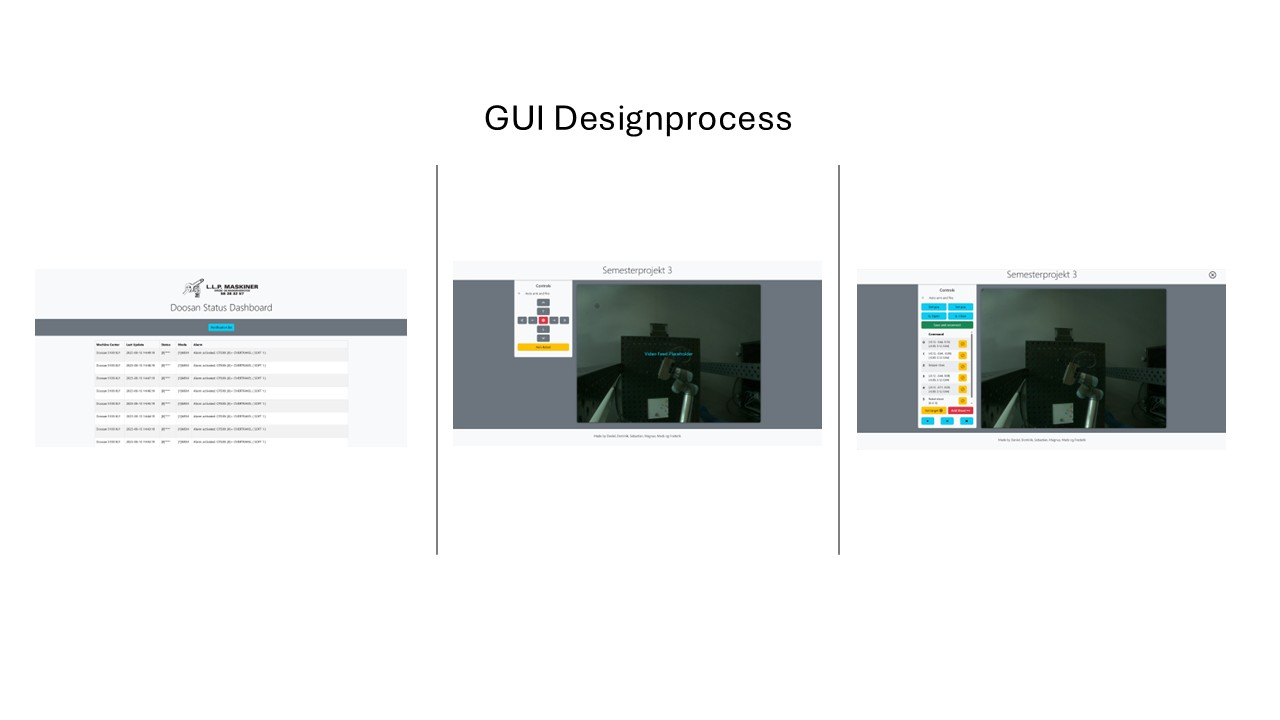
\includegraphics[width=190mm,center]{figures/GUI designprocess.jpg}

Later when we got the automatic functions up and running(The pick up ball function and the find box function)), the grapics changed somewhat. Instead of you had to click the target and then click set position, it was automaticly made to set position, so we could free up a button.
That meant we could add find ball in manual mode. So here the only difference was you had to pick your target yourself. This is also used heavily in the tests.

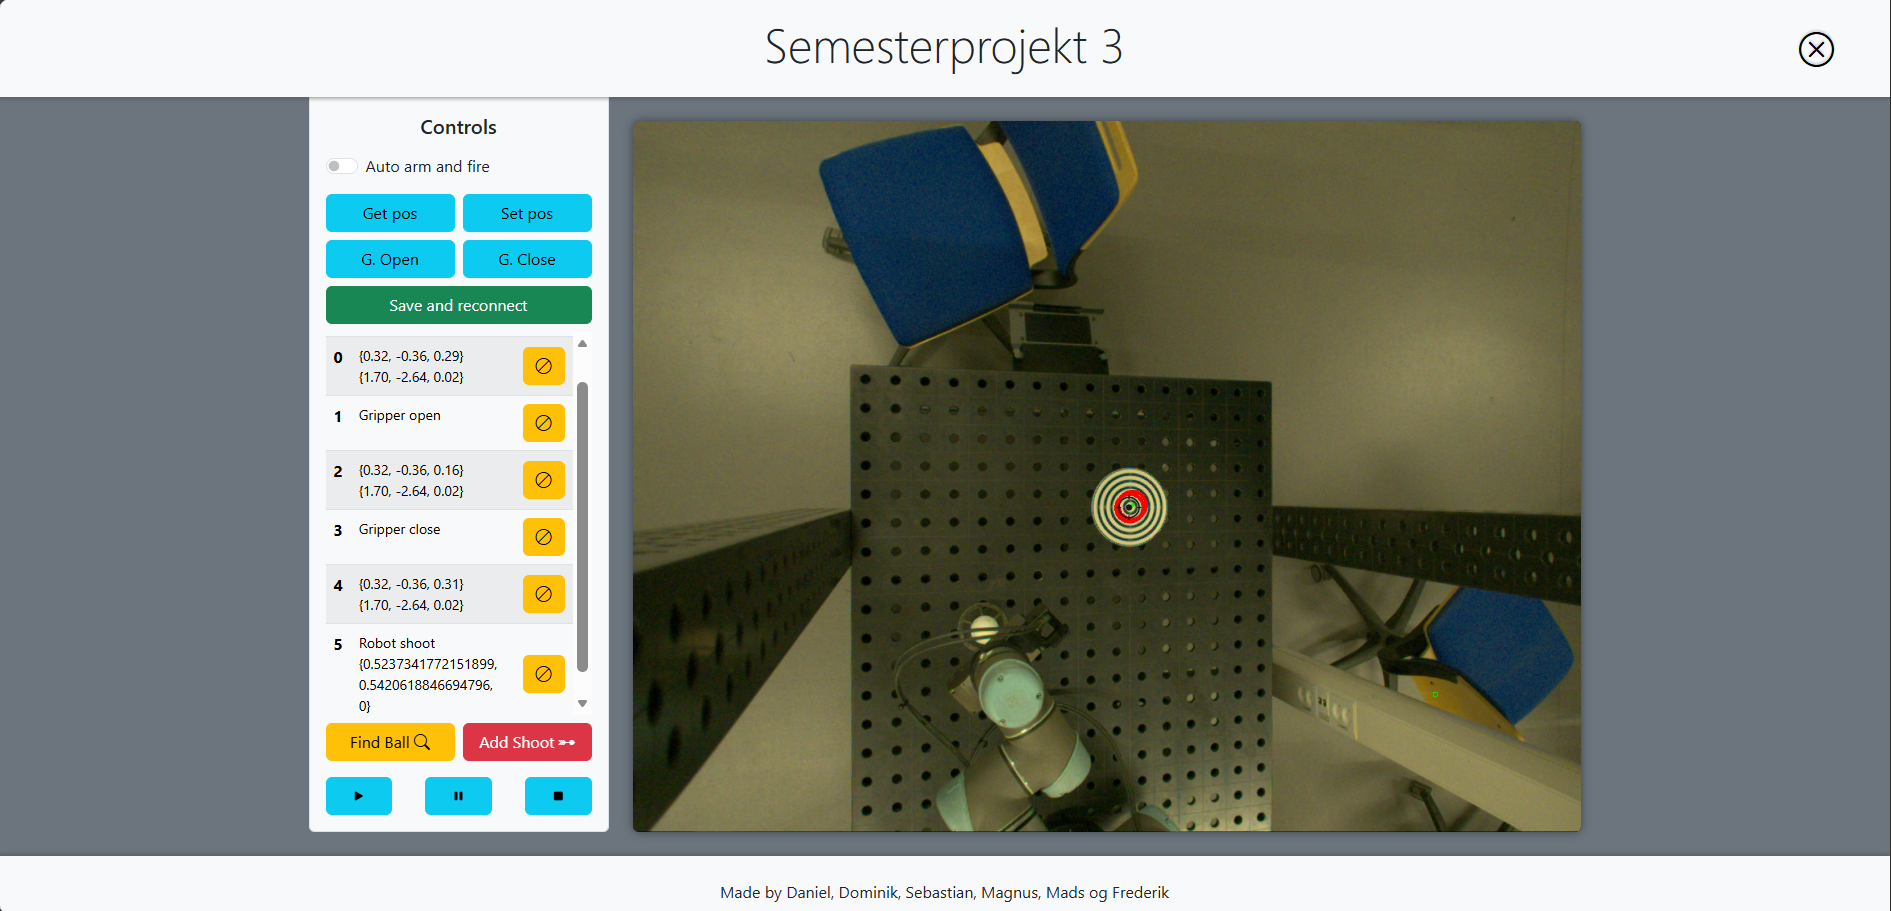
\includegraphics[width=190mm,center]{figures/GUI finalDesign.png}




\newpage

\section{Implementation} 
\label{sec:Implementation}

\subsection{Integration}
The GUI is tightly linked with the robotControl, so as we came forward and the GUI was almost done, robotControl and GUI teamed up.
The GUI runs primarily in the main loop, QT is being given the main loop at app.exec(). 
We setup the GUI webpage in the webPage class and the rest in at appSetup.cpp.
Because Qt disallow GUI outside the main loop, you have to use signals to deliver the message which is why there is a MsgSender class.
To use the MsgSender class you have to add a link to the main thread, again to run it in the main thread, which is being done in the appSetup.cpp which is setup and exit script.

The main implementation happens in the QThread class that runs a loop, which control the robot. The website sends signals from the main thread that the robot thread will use and answer.

To make the website work in robotControl, the URThreadControl loop really runs the entire function of the application. 
It is here we tell the robot to run the commands, the website has given. It is here we tell the website, where it is the robot is at right now, so you can create commands for later use.
It is the core of the program. Here it is parted up into two different loops. Either we run in auto, where we ask cameravision where we want to go or we manually create commands that the robot can follow. 
-Later the automatic commands was added to manually also.

Because everyone else in the group works in world coordinates and the robot does not, a kinematics library has been created to work between them along with the WORLD\_TO\_BASE and BASE\_TO\_WORLD transformation matrix. 
This lib is also used to change between UR axis angles and transformation matrixes. This is how we calculate where we are in the world coordinates and where we need to go.

The Vision part is copied directly into main and the videofeed transfered to the webpage GUI through another thread.

The matlab script, which runs the trajectory calculations, is integrated into a throw command in robotControl. \- So when called, It will calculate trajectories and follow them.

We do run quite alot of threads which can and do cause quite some issues. This was of cause not an issue while the programs were seperate. The issue is that we need to connect different variables To fix this we do use quite alot of mutexes and atomics. These make sure that no thread can write to a thread being used by another thread.
This was all needed to make an application that would be responsive.
RobotControl is always being called from the browser to tell which commands to run. RobotControl launches another thread when shooting to make sure it has the highest priority, to make the throw move without stops. The throw also launches a thread more to make sure that the gripper releases at the right time.
Beyond that, the vision tells the browser what image to show, while at the same time finding different objects in the image. The image in the browser also has its own thread, because it requires mjpeg streamer, which is a library to stream the vision.

This all together creates a responsive app that just works!

Even though it is a little illigal, there are two gotos in this loop. One restarts the loop if you have asked to "save and reconnect". 
This exits everything in this loop and saves the commands you are following. Then it reboots the loop from top.
Another goto is there to exit the deep loops. When it is not enough just to break out of a loop. This is for example when you are searching for a ball and wanting to stop the search. 
This would only break out into the normal loop and we would continue and move to a ball we did not find.
These could be solved in other ways. But i believe this was the easiest and best solution to this problem.


\subsection{Usage}

\begin{itemize}
\item In the control panel on the left on top, there is a slider. 
This slider desides whether you are running in automatic mode or in manual mode.
if you are in auto you can only control play, pause and stop.
if not, you can use the rest of the control panel. You can add elements to the loop and start, pause and stop the loop.
These elements are "Set position", "Gripper open", "Gripper close", "Find ball" and "Add shoot".
Along with that, there is a "Get position" to get the coordinates in UR axis angles and "Save and reconnect". 

\begin{itemize}
\item With "Set position", you can set a position, you have moved it to on the teachpendent. 
\item "Gripper open" and "Gripper close" tells the loop to open and close the gripper.
\item "Find ball" is the newest member function. It tells to get the cameravision to find the ball where it is. This changes every loop. So the function does not set any target points directly.
\item "Add shoot" uses the coordinates you have picked on the table. Click on the table on the videofeed, to select a target.
\end{itemize}

\item In the right top corner there is a shutdown button. This button can be used to safely quit all threads and exit.

\item If you close the tab in error, you can find in the taskbar, the logo being presented. By double clicking on the logo, you will be able to open the website.
If you right click, you can shut down the program safely.

\end{itemize}
\newpage

\section{Evaluation} 
\subsection{Getting speedJ to work}
SpeedJ changes the speeds the every joint down the kinematic chain. This means we get a more flowing motion, however it comes at a cost. - Precision. 
\newline We have to update at the precise time to fit the speeds.
\newline A way of illustrating this would be Eulers method to first order differential equations. 
\newline Here everything is a little off as we always approximate with the tangent. This will get more and more off the real target the larger steps you take. 
\newline The same is true for this. This is actually really much the same.\newline

Another problem we will show is that we do not reach the targets we want to by using servoJ or moveL. there is an offset. Note that we are giving it a point it should be and reading out where it arrived at.
\newline This could mean that it takes in some offset to counterbalance the its own weight. However i do not know this. This is just me thinking.\newline

For the sake of reducing the text, i will only show the first and the last step in the record. For the full record i will give the path to the test.
\newline All of the tests is in radians. TimeStep is in seconds.
\newline These tests are done in simulation only if nothing else is noted.
\subsubsection{Raw speedJ with servoJ to get to startpoint}
Here we are trying to take a look at the problem. 
\newline As you can see. We are starting off. And even though these test are done precisely same, they start in different points. properly because of the wobble. We are waiting 3 seconds here to reduce wobble.
\newline Also the servoJ has some offset. 
\newline Here we are using servoJ to position us to the first point and using speedJ from there:

\paragraph{test1}
Full test at "tests/throwCalculationsTests/speedJTests/Test1.txt"\newline

start of test:\newline

throwPositions with timeStep:  0.05
\newline new throwPositions is a vector X: 41 Y:  6
\newline new recoveryPositions is a vector X: 21 Y:  6
\newline Thread priority is: Time Critical
\newline [0.000000s - Step 0/41]:
\newline \hspace{1cm}        pos(-1.313193, -1.579761, -1.450452, -0.220422, 1.501750, -0.064856) should be:
\newline \hspace{1cm}        pos(-1.178097, -1.570796, -1.265364, -0.087266, 1.483530, 0.000000)
\newline [2.000000s - Step 40/41]:
\newline \hspace{1cm}        pos(-1.447671, -1.822501, -1.549878, -1.323733, 1.550060, -0.258894) should be:
\newline \hspace{1cm}        pos(-1.379977, -1.871966, -1.389736, -1.450072, 1.569761, -0.203377)\newline

end of test.\newline

As you can see if we are not even hitting the position in servoJ. It is also noted that the robot stands and wobbles.\newline

positon error in the begging is pos(-0.135096, -0.008965, -0.185088, -0.136954, 0.01822, -0.064856)
\newline positon error in the end is pos(-0.067694, -0.049465, -0.160042, 0.126339, -0.019701, -0.055517)\newline 

\paragraph{test2}
Full test at "tests/throwCalculationsTests/speedJTests/Test2.txt"\newline

start of test:\newline

throwPositions with timeStep:  0.05
\newline new throwPositions is a vector X: 41 Y:  6
\newline new recoveryPositions is a vector X: 21 Y:  6
\newline Thread priority is: Time Critical
\newline [0.000000s - Step 0/41]:
\newline \hspace{1cm}        pos(-1.307165, -1.579367, -1.442189, -0.214486, 1.500933, -0.061969) should be:
\newline \hspace{1cm}        pos(-1.178097, -1.570796, -1.265364, -0.087266, 1.483530, 0.000000)
\newline [2.000000s - Step 40/41]:
\newline \hspace{1cm}        pos(-1.442427, -1.816584, -1.539463, -1.292029, 1.551028, -0.247493) should be:
\newline \hspace{1cm}       pos(-1.379977, -1.871966, -1.389736, -1.450072, 1.569761, -0.203377)\newline

end of test.\newline 

As you can see if we are not even hitting the position in servoJ. It is also noted that the robot stands and wobbles.\newline

positon error in the begging is pos(-0.129068, -0.008571, -0.176825, -0.127220, 0.017403, -0.061969)
\newline positon error in the end is pos(-0.062450, 0.055382, -0.149727, 0.158043, -0.018733, -0.044116)

\paragraph{Notes from tests}
As you can see there is a difference in start position of the two tests. The difference is pos(-0.006028, -0.000394, -0.008263, -0.009734, 0.000817, -0.002887), which is just weird. But small enough to be negligible.
\newline Also you can see there is a very big difference in where we want to be in the begging and where we end up. Note that this in radians and a very small step means a whole lot.\newline

converted to degrees, you can clearly see the picture:
\newline test 1 start: pos(-7.740431, -0.513657, -10.604761, -7.846886, 1.043929, -3.715975) degrees.
\newline test 2 start: pos(-7.395052, -0.491082, -10.131326, -7.289169, 0.997118, -3.550562) degrees.\newline 

This is really alot and is NOT negligible.

The average of these two start positions is pos(-1.310179, -1.579564, -1.446321, -0.217454, 1.501342, -0.063413). \newline 
The error from this is pos(-0.132082, -0.008768, -0.180957, -0.130188, 0.017812, -0.063413).
\newline We will use this in the next tests.

\subsubsection{Raw speedJ with TM to get to startpoint and a moveL}
To get a clearer picture of why we are so much off in start position from where we want to be, we will try using a craigs DH parameters and generating a TM and converting to UR axis angles and use moveL to position us.

\paragraph{test1}
Full test at "tests/throwCalculationsTests/speedJTests/TestMedTMsomStart/Test1.txt"\newline

start of test:\newline

throwPositions with timeStep:  0.05
\newline new throwPositions is a vector X: 41 Y:  6
\newline new recoveryPositions is a vector X: 21 Y:  6
\newline Thread priority is: Time Critical
\newline [0.000000s - Step 0/41]:
\newline \hspace{1cm}        pos(-1.328631, -1.651214, -1.119946, -0.152718, 1.630515, 0.032523) should be:
\newline \hspace{1cm}        pos(-1.178097, -1.570796, -1.265364, -0.087266, 1.483530, 0.000000)
\newline [2.000000s - Step 40/41]:
\newline \hspace{1cm}        pos(-1.480086, -1.921114, -1.230553, -1.379144, 1.685679, -0.181168) should be:
\newline \hspace{1cm}       pos(-1.379977, -1.871966, -1.389736, -1.450072, 1.569761, -0.203377)\newline 

end of test.\newline 

\paragraph{test2}
Full test at "tests/throwCalculationsTests/speedJTests/TestMedTMsomStart/Test2.txt"\newline

start of test:\newline

throwPositions with timeStep:  0.05
\newline new throwPositions is a vector X: 41 Y:  6
\newline new recoveryPositions is a vector X: 21 Y:  6
\newline Thread priority is: Time Critical
\newline [0.000000s - Step 0/41]:
\newline \hspace{1cm}        pos(-1.328631, -1.651214, -1.119946, -0.152718, 1.630515, 0.032523) should be:
\newline \hspace{1cm}        pos(-1.178097, -1.570796, -1.265364, -0.087266, 1.483530, 0.000000)
\newline [2.000000s - Step 40/41]:
\newline \hspace{1cm}        pos(-1.482983, -1.916780, -1.228931, -1.358526, 1.688793, -0.172052) should be:
\newline \hspace{1cm}        pos(-1.379977, -1.871966, -1.389736, -1.450072, 1.569761, -0.203377)

end of test.\newline 

\paragraph{Notes from tests}
The wobble is totally gone. Now we have reduced the problem in startposition to pos(0.0, 0.0, 0.0, 0.0, 0.0, 0.0)\newline 

Difference end pos(0.002897, -0.004334, -0.001622, -0.020618, -0.003114, -0.009116) between test1 and test2 -> Converted to degrees: pos(0.165986, -0.248320, -0.092934, -1.181324, -0.178419, -0.522308)\newline 

This however does not change the problem with the start offset which is very clear here.
\newline difference in start position for both test1 and test2: pos(-0.150534, -0.080418, 0.145418, -0.065452, 0.146985, 0.032523) -> Converted to degrees: pos(-8.624963, -4.607612, 8.331838, -3.750123, 8.421620, 1.863431)\newline 

and from previous test start average, we can see a change in position on pos(0.018452, 0.071650, -0.326375, -0.064736, -0.129173, -0.095936) which means we are not offseting precisely the same target as we did before. \newline 
But it still confirms we are trying to reach the same target. This can still be the wobble or the a rounding error, but i do not know.

\subsubsection{Raw speedJ with payload activated with TM to get to startpoint and a moveL}
To get a clearer picture of why we are so much off in start position we will try changing payload.\newline 

In simulation there is a payload of 0.0Kg at the beginning

\paragraph{test1}
Full test at "tests/throwCalculationsTests/speedJTests/TestMedTMogPayload2.85Aktiveret/test1.txt"\newline 

start of test:\newline 

throwPositions with timeStep:  0.05
\newline new throwPositions is a vector X: 41 Y:  6
\newline new recoveryPositions is a vector X: 21 Y:  6
\newline Thread priority is: Time Critical
\newline [0.000000s - Step 0/41]:
\newline \hspace{1cm}        pos(-1.328631, -1.651214, -1.119946, -0.152718, 1.630515, 0.032523) should be:
\newline \hspace{1cm}        pos(-1.178097, -1.570796, -1.265364, -0.087266, 1.483530, 0.000000)
\newline [2.000000s - Step 40/41]:
\newline \hspace{1cm}        pos(-1.482096, -1.920982, -1.230559, -1.378185, 1.687216, -0.178841) should be:
\newline \hspace{1cm}        pos(-1.379977, -1.871966, -1.389736, -1.450072, 1.569761, -0.203377)\newline 

end of test.\newline 

\paragraph{Notes from tests}
As you can see it has no difference in startposition from before. The difference between "tests/throwCalculationsTests/speedJTests/TestMedTMsomStart/Test2.txt" and this test "tests/throwCalculationsTests/speedJTests/TestMedTMogPayload2.85Aktiveret/test1.txt", is pos(0.0, 0.0, 0.0, 0.0, 0.0, 0.0). \newline 

We can conclude that the function of payload changes nothing. Also we can read on URs website that payload is used to make sure the robots emergency stop is not activated when carrying heavy objects. 
\newline - https://www.universal-robots.com/manuals/EN/HTML/SW5\_20/Content/prod-usr-man/complianceUR5e/SW\_sections/first\_program/payload\_set.htm\newline 

Though i still believe this offset is due to counterbalancing the weight of the robot. 
\newline Another thought might be that it does not compensate for payload on the simulation. - I do not believe so, but it is hard to find anything on it. 
\newline It would be stupid if it compensated for the robots weight but not for the payload in the simulation only.

Another hint is setGravity function which set the direction of gravity, so there is clearly something here. \newline

\subsubsection{Another test of raw speedJ with payload activated with TM to get to startpoint and a moveL}
To be sure i did the test again with different positions. 
\newline This is done later so the output is suddenly a little different, but it will be clearer in the later test as why. \newline 

In this test i will first test with 0Kg and later with 5Kg

\paragraph{test1}
Full test at "tests/throwCalculationsTests/speedJTests/LaterTestMedTMogPayloadChange/test1.txt"

start of test: \newline 

throwPositions with timeStep:  0.008
\newline new throwPositions is a vector X: 126 Y:  6
\newline new recoveryPositions is a vector X: 126 Y:  6
\newline Payload is:  0  Kg
\newline Thread priority is: Time Critical
\newline [0.000000s - Step 0/126]:
\newline \hspace{1cm}        pos(-1.328631, -1.651214, -1.119946, -0.152718, 1.630515, 0.032523) should be:
\newline \hspace{1cm}        pos(-1.178097, -1.570796, -1.265364, -0.087266, 1.483530, 0.000000)
\newline \hspace{1cm}        posError: (-0.150534, -0.080418, 0.145417, -0.065451, 0.146985, 0.032523)
\newline \hspace{1cm}        speed: (-0.001768, -0.012633, -0.007734, -0.064238, 0.010466, -0.012998)
\newline \hspace{1cm}        speedCorrection: (0.000000, 0.000000, 0.000000, 0.000000, 0.000000, 0.000000)
\newline [1.000000s - Step 125/126]:
\newline \hspace{1cm}        pos(-1.440319, -1.955422, -1.353232, -1.764022, 1.725888, -0.169566) should be:
\newline \hspace{1cm}        pos(-1.316706, -1.839975, -1.431652, -1.440214, 1.569724, -0.140117)
\newline \hspace{1cm}        posError: (-0.123613, -0.115447, 0.078420, -0.323808, 0.156164, -0.029450)
\newline \hspace{1cm}        speedCorrection: (-3.135285, -2.863931, 2.034452, -7.874681, 3.904035, -0.670984)

end of test.\newline 

\paragraph{test2}
Full test at "tests/throwCalculationsTests/speedJTests/LaterTestMedTMogPayloadChange/test2.txt"

start of test: \newline 

throwPositions with timeStep:  0.008
\newline new throwPositions is a vector X: 126 Y:  6
\newline new recoveryPositions is a vector X: 126 Y:  6
\newline Payload is:  5  Kg
\newline Thread priority is: Time Critical
\newline[0.000000s - Step 0/126]:
\newline \hspace{1cm}        pos(-1.328631, -1.651214, -1.119946, -0.152718, 1.630515, 0.032523) should be:
\newline \hspace{1cm}        pos(-1.178097, -1.570796, -1.265364, -0.087266, 1.483530, 0.000000)
\newline \hspace{1cm}        posError: (-0.150534, -0.080418, 0.145417, -0.065451, 0.146985, 0.032523)
\newline \hspace{1cm}        speed: (-0.001768, -0.012633, -0.007734, -0.064238, 0.010466, -0.012998)
\newline \hspace{1cm}        speedCorrection: (0.000000, 0.000000, 0.000000, 0.000000, 0.000000, 0.000000)
\newline[1.000000s - Step 125/126]:
\newline \hspace{1cm}        pos(-1.378436, -1.918691, -1.404294, -1.707772, 1.670588, -0.180884) should be:
\newline \hspace{1cm}        pos(-1.316706, -1.839975, -1.431652, -1.440214, 1.569724, -0.140117)
\newline \hspace{1cm}        posError: (-0.061730, -0.078716, 0.027358, -0.267558, 0.100864, -0.040767)
\newline \hspace{1cm}        speedCorrection: (-1.648650, -1.986026, 0.796333, -6.560566, 2.568193, -0.945082)

end of test.\newline 

\paragraph{Notes from tests}
As you can see it has no difference in startposition from before and the payload clearly changes.\newline

\subsubsection{Errorcorrection in speedJ and moveJ instead of moveL or servoJ}
We found that if we changed moveL/servoJ to moveJ, we did not have this offset as previously found. So that made us use moveJ.\newline
Another error we have is correcting the speed at the right time to reach the correct position.\newline

In these tests we have both videoes of the real robot and tests in simulations. There are really many tests, so only a few will be presented here.

\paragraph{test1}
Full test at "tests/throwCalculationsTests/speedJTests/TestMedMoveJSomStart/test1.txt"

Here we do not change the position yet. \newline

start of test: \newline 

throwPositions with timeStep:  0.008\newline 
new throwPositions is a vector X: 251 Y:  6\newline 
new recoveryPositions is a vector X: 126 Y:  6\newline 
Thread priority is: Time Critical\newline 
[0.000000s - Step 0/251]:\newline 
\hspace{1cm}        pos(-1.178097, -1.570796, -1.265364, -0.087266, 1.483530, 0.000000) should be:\newline 
\hspace{1cm}         pos(-1.178097, -1.570796, -1.265364, -0.087266, 1.483530, 0.000000)\newline 
\hspace{1cm}         posError: (0.000000, 0.000000, 0.000000, 0.000000, -0.000000, 0.000000)\newline 
[2.000000s - Step 250/251]:\newline 
\hspace{1cm}         pos(-1.348720, -1.837965, -1.375449, -1.297685, 1.553672, -0.189447) should be:\newline 
\hspace{1cm}         pos(-1.379977, -1.871966, -1.389736, -1.450072, 1.569761, -0.203377)\newline 
\hspace{1cm}         posError: (0.031258, 0.034001, 0.014286, 0.152387, -0.016089, 0.013930)\newline 

end of test.\newline 

The resulting error in degrees is: (1.791, 1.949, 0.818, 8.732, -0.922, 0.798). This is quite alot different from where we want to be.

\paragraph{test4 with correction}
Full test at "tests/throwCalculationsTests/speedJTests/TestMedMoveJSomStart/test4Correction.txt"

Here we change the positions. \newline 

start of test: \newline 

throwPositions with timeStep:  0.008\newline
new throwPositions is a vector X: 251 Y:  6\newline
new recoveryPositions is a vector X: 126 Y:  6\newline
Thread priority is: Time Critical\newline
[0.000000s - Step 0/251]:\newline
\hspace{1cm}        pos(-1.178097, -1.570796, -1.265364, -0.087266, 1.483530, 0.000000) should be:\newline
\hspace{1cm}        pos(-1.178097, -1.570796, -1.265364, -0.087266, 1.483530, 0.000000)\newline
\hspace{1cm}        posError: (0.000000, 0.000000, 0.000000, 0.000000, -0.000000, 0.000000)
\hspace{1cm}        speed: (0.001307, -0.003422, -0.001309, -0.016111, -0.001723, -0.006153)\newline
\hspace{1cm}        speedCorrection: (0.000000, 0.000000, 0.000000, 0.000000, 0.000000, 0.000000)\newline
[2.000000s - Step 250/251]:\newline
\hspace{1cm}        pos(-1.376371, -1.872063, -1.389670, -1.451151, 1.567033, -0.207359) should be:\newline
\hspace{1cm}        pos(-1.379977, -1.871966, -1.389736, -1.450072, 1.569761, -0.203377)\newline
\hspace{1cm}        posError: (0.003606, -0.000097, 0.000066, -0.001078, -0.002728, -0.003982)\newline
\hspace{1cm}        speedCorrection: (0.050581, -0.000597, 0.001231, -0.011548, -0.038093, -0.054787)\newline

end of test.\newline 

The resulting error in degrees is: (0.207, -0.006, 0.004, -0.062, -0.156, -0.228). This is much better.

\paragraph{test5 on the real robot}
Full test at "tests/throwCalculationsTests/speedJTests/TestMedMoveJSomStart/test5OnRealRobot.txt"

This is a test on the real robot. The test is executed on Ubuntu.

start of test: \newline 

throwPositions with timeStep:  0.008\newline 
new throwPositions is a vector X: 251 Y:  6\newline 
new recoveryPositions is a vector X: 126 Y:  6\newline 
Thread priority is: \newline 
Policy: SCHED\_FIFO, Priority: 95\newline 
[Vision detection]: 69.0066 26.2165\newline 

Connected successfully to: 192.168.1.11 at 30004\newline 
RTDE synchronization started\newline 
[Vision detection]: 78.5706 21.9786\newline 

[0,000000s - Step 0/251]:\newline 
\hspace{1cm}	pos(-1,178128, -1,570760, -1,265427, -0,087320, 1,483462, -0,000048) should be: \newline 
\hspace{1cm}	pos(-1,178097, -1,570796, -1,265364, -0,087266, 1,483530, 0,000000)\newline 
\hspace{1cm}	posError: (-0,000030, 0,000036, -0,000063, -0,000053, -0,000067, -0,000048)\newline 
\hspace{1cm}	speed: (0,000516, -0,002887, -0,002129, -0,015988, -0,003211, -0,002876)\newline 
\hspace{1cm}	speedCorrection: (0,000000, 0,000000, 0,000000, 0,000000, 0,000000, 0,000000)\newline 
[2,000000s - Step 250/251]:\newline 
\hspace{1cm}	pos(-1,279345, -1,824083, -1,454792, -1,441599, 1,575537, -0,097324) should be: \newline 
\hspace{1cm}	pos(-1,275991, -1,822698, -1,453854, -1,435333, 1,569703, -0,099401)\newline 
\hspace{1cm}	posError: (-0,003354, -0,001385, -0,000939, -0,006265, 0,005834, 0,002078)\newline 
\hspace{1cm}	speedCorrection: (-0,052390, -0,019909, -0,014895, -0,083673, 0,085495, 0,029314)\newline 

end of test.\newline 

The resulting error in degrees is: (-0.192, -0.079, -0.054, -0.359, 0.334, 0.119). This is much better.

\paragraph{test6 on the real robot}
Full test at "tests/throwCalculationsTests/speedJTests/TestMedMoveJSomStart/test6OnRealRobot.txt"

This is a test on the real robot. The test is executed on Ubuntu.

start of test: \newline 

throwPositions with timeStep:  0.008\newline 
new throwPositions is a vector X: 251 Y:  6\newline 
new recoveryPositions is a vector X: 126 Y:  6\newline 
Thread priority is: \newline 
Policy: SCHED\_FIFO, Priority: 95\newline 

[0,000000s - Step 0/251]:\newline 
\hspace{1cm}	pos(-1,178091, -1,570808, -1,265391, -0,087283, 1,483450, 0,000048) should be:\newline  
\hspace{1cm}	pos(-1,178097, -1,570796, -1,265364, -0,087266, 1,483530, 0,000000)\newline 
\hspace{1cm}	posError: (0,000006, -0,000012, -0,000027, -0,000017, -0,000079, 0,000048)\newline 
\hspace{1cm}	speed: (0,002586, -0,002739, -0,003498, -0,016350, -0,006692, 0,001787)\newline 
\hspace{1cm}	speedCorrection: (0,000000, 0,000000, 0,000000, 0,000000, 0,000000, 0,000000)\newline 
[1,512000s - Step 189/251]:\newline 
\hspace{1cm}	pos(-1,007477, -1,751977, -1,500767, -1,242321, 1,287545, 0,142233) should be: \newline 
\hspace{1cm}	pos(-1,008157, -1,751160, -1,499759, -1,236134, 1,285925, 0,141296)\newline 
\hspace{1cm}	posError: (0,000680, -0,000817, -0,001008, -0,006187, 0,001620, 0,000936)\newline 
\hspace{1cm}	speed: (0,090148, -0,096191, -0,130956, -0,719353, 0,253719, 0,110214)\newline 
\hspace{1cm}	speedCorrection: (-0,000061, 0,000446, 0,001573, -0,003420, -0,003991, 0,000369)\newline 
[1,520000s - Step 190/251]:\newline 
\hspace{1cm}	pos(-1,007477, -1,751977, -1,500767, -1,242321, 1,287545, 0,142233) should be: \newline 
\hspace{1cm}	pos(-1,007429, -1,751936, -1,500815, -1,241924, 1,287918, 0,142181)\newline 
\hspace{1cm}	posError: (-0,000048, -0,000041, 0,000048, -0,000397, -0,000373, 0,000052)\newline 
\hspace{1cm}	speed: (0,088489, -0,094440, -0,128806, -0,710442, 0,263167, 0,109574)\newline 
\hspace{1cm}	speedCorrection: (0,008501, -0,010216, -0,012606, -0,077338, 0,020247, 0,011705)\newline 
[1,528000s - Step 191/251]:\newline 
\hspace{1cm}	pos(-1,007477, -1,751977, -1,500767, -1,242321, 1,287545, 0,142233) should be: \newline 
\hspace{1cm}	pos(-1,006715, -1,752699, -1,501854, -1,247644, 1,289985, 0,143060)\newline 
\hspace{1cm}	posError: (-0,000762, 0,000722, 0,001087, 0,005322, -0,002440, -0,000827)\newline 
\hspace{1cm}	speed: (0,086808, -0,092667, -0,126627, -0,701398, 0,272700, 0,108921)\newline 
\hspace{1cm}	speedCorrection: (-0,000595, -0,000511, 0,000596, -0,004962, -0,004656, 0,000653)\newline 
[1,536000s - Step 192/251]:\newline 
\hspace{1cm}	pos(-1,007477, -1,751977, -1,500767, -1,242321, 1,287545, 0,142233) should be: \newline 
\hspace{1cm}	pos(-1,006014, -1,753447, -1,502876, -1,253291, 1,292128, 0,143934)\newline 
\hspace{1cm}	posError: (-0,001463, 0,001470, 0,002108, 0,010970, -0,004583, -0,001701)\newline 
\hspace{1cm}	speed: (0,085104, -0,090869, -0,124418, -0,692221, 0,282317, 0,108256)\newline 
\hspace{1cm}	speedCorrection: (-0,009528, 0,009021, 0,013584, 0,066529, -0,030500, -0,010337)\newline 
[1,544000s - Step 193/251]:\newline 
\hspace{1cm}	pos(-1,007477, -1,751977, -1,500767, -1,242321, 1,287545, 0,142233) should be: \newline 
\hspace{1cm}	pos(-1,005326, -1,754182, -1,503880, -1,258866, 1,294348, 0,144803)\newline 
\hspace{1cm}	posError: (-0,002151, 0,002204, 0,003113, 0,016544, -0,006803, -0,002570)\newline 
\hspace{1cm}	speed: (0,083378, -0,089049, -0,122179, -0,682911, 0,292020, 0,107578)\newline 
\hspace{1cm}	speedCorrection: (-0,018293, 0,018376, 0,026356, 0,137122, -0,057293, -0,021262)\newline 
RTDEControlInterface: RTDE control script is not running!\newline 
[1,824000s - Step 228/251]:\newline 
\hspace{1cm}	pos(-1,007477, -1,751977, -1,500767, -1,242321, 1,287545, 0,142233) should be: \newline 
\hspace{1cm}	pos(-0,991177, -1,769410, -1,526121, -1,399795, 1,425589, 0,171091)\newline 
\hspace{1cm}	posError: (-0,016300, 0,017432, 0,025353, 0,157473, -0,138044, -0,028859)\newline 
\hspace{1cm}	speed: (0,008892, -0,010432, -0,025097, -0,273308, 0,685133, 0,075788)\newline 
\hspace{1cm}	speedCorrection: (-0,202488, 0,216466, 0,313918, 1,938998, -1,658932, -0,352985)\newline 
[2,000000s - Step 250/251]:\newline 
\hspace{1cm}	pos(-1,007477, -1,751977, -1,500767, -1,242321, 1,287545, 0,142233) should be: \newline 
\hspace{1cm}	pos(-0,994322, -1,766273, -1,524373, -1,421563, 1,569606, 0,182280)\newline 
\hspace{1cm}	posError: (-0,013156, 0,014296, 0,023606, 0,179241, -0,282061, -0,040047)\newline 
\hspace{1cm}	speedCorrection: (-0,169189, 0,183601, 0,299944, 2,244743, -3,429387, -0,495603)\newline 

end of test.\newline 

The resulting error in degrees is: (-0.754°, 0.819°, 1.353°, 10.273°, -16.160°, -2.295°). This is much worse. \newline 
The problem here being that we hit protective stop quite often. This is a fight the group was having over a long time. Why these happens we were forever fighting about. \newline 
As you can see the error is exploding from 1.5s. So i suspect that the protective stop has already been hit here.\newline 

for more information, check the file.\newline 

\paragraph{test7 on the real robot}
Full test at "tests/throwCalculationsTests/speedJTests/TestMedMoveJSomStart/test7"

This is a test on the real robot. The test is executed on Windows.

\textbf{This test include a video}

start of test: \newline 

throwPositions with timeStep:  0.008\newline
new throwPositions is a vector X: 251 Y:  6\newline
new recoveryPositions is a vector X: 126 Y:  6\newline
Thread priority is: Time Critical\newline
[0.000000s - Step 0/251]:\newline
\hspace{1cm}        pos(-1.178140, -1.570808, -1.265379, -0.087332, 1.483450, 0.000024) should be:\newline
\hspace{1cm}        pos(-1.178097, -1.570796, -1.265364, -0.087266, 1.483530, 0.000000)\newline
\hspace{1cm}        posError: (-0.000042, -0.000012, -0.000016, -0.000065, -0.000079, 0.000024)\newline
\hspace{1cm}        speed: (0.002573, -0.002744, -0.003503, -0.016355, -0.006792, 0.001799)\newline
\hspace{1cm}        speedCorrection: (0.000000, 0.000000, 0.000000, 0.000000, 0.000000, 0.000000)\newline
[2.000000s - Step 250/251]:\newline
\hspace{1cm}        pos(-0.990166, -1.771110, -1.529706, -1.441071, 1.537483, 0.182963) should be:\newline
\hspace{1cm}        pos(-0.994327, -1.766273, -1.524373, -1.421563, 1.569606, 0.182272)\newline
\hspace{1cm}        posError: (0.004160, -0.004837, -0.005333, -0.019508, -0.032123, 0.000691)\newline
\hspace{1cm}        speedCorrection: (0.051757, -0.059545, -0.065179, -0.243162, -0.381999, 0.008985)\newline

end of test.\newline 

The resulting error in degrees is: (0.238, -0.277, -0.305, -1.118, -1.841, 0.040). This is better, but worse than the first test. This can because of the lag. Check video.

\paragraph{test8 on the real robot} 
Invalid. Starts in wrong position. Properly running an old test.

timeStep has been changed to 0.1s\newline
This is a test on the real robot. The test is executed on Windows.\newline

\textbf{This test include a video}\newline

\paragraph{test9 on the real robot}
Full test at "tests/throwCalculationsTests/speedJTests/TestMedMoveJSomStart/Test9"

This is a test on the real robot. The test is executed on Windows.\newline
timeStep has been changed to 0.1s\newline
Gain on the speedCorrection has been changed from 0.2 back to 0.1

\textbf{This test include a video}

start of test: \newline 

throwPositions with timeStep:  0.1\newline 
new throwPositions is a vector X: 21 Y:  6\newline 
new recoveryPositions is a vector X: 11 Y:  6\newline 
Thread priority is: Time Critical\newline 
[0.000000s - Step 0/21]:\newline 
\hspace{1cm}         pos(-1.178032, -1.570760, -1.265415, -0.087283, 1.483535, 0.000084) should be:\newline 
\hspace{1cm}         pos(-1.178097, -1.570796, -1.265364, -0.087266, 1.483530, 0.000000)\newline 
\hspace{1cm}         posError: (0.000065, 0.000036, -0.000051, -0.000017, 0.000005, 0.000084)\newline 
\hspace{1cm}         speed: (0.030572, -0.032599, -0.041652, -0.194881, -0.078709, 0.021564)\newline 
\hspace{1cm}         speedCorrection: (0.000000, 0.000000, 0.000000, 0.000000, 0.000000, 0.000000)\newline 
[2.000000s - Step 20/21]:
\hspace{1cm}         pos(-0.985183, -1.775944, -1.536269, -1.465828, 1.492436, 0.183981) should be:\newline 
\hspace{1cm}         pos(-0.994327, -1.766273, -1.524373, -1.421563, 1.569606, 0.182274)\newline 
\hspace{1cm}         posError: (0.009144, -0.009671, -0.011895, -0.044265, -0.077169, 0.001707)\newline 
\hspace{1cm}         speedCorrection: (0.007085, -0.007576, -0.009098, -0.035438, -0.051935, 0.001812)\newline 
 
end of test.\newline 

The resulting error in degrees is: (0.524°, -0.554°, -0.681°, -2.536°, -4.421°, 0.098°). This is nearly as bad as without.\newline 

There is also a simulation of this throw:\newline 

start of test: \newline 

throwPositions with timeStep:  0.1\newline 
new throwPositions is a vector X: 21 Y:  6\newline 
new recoveryPositions is a vector X: 11 Y:  6\newline 
Thread priority is: Time Critical\newline 
[0.000000s - Step 0/21]:\newline 
\hspace{1cm}        pos(-1.178097, -1.570796, -1.265364, -0.087266, 1.483530, 0.000000) should be:\newline 
\hspace{1cm}        pos(-1.178097, -1.570796, -1.265364, -0.087266, 1.483530, 0.000000)\newline 
\hspace{1cm}        posError: (0.000000, 0.000000, 0.000000, 0.000000, -0.000000, 0.000000)\newline 
\hspace{1cm}        speed: (0.014508, -0.040853, -0.015659, -0.192136, -0.019744, -0.072274)\newline 
\hspace{1cm}        speedCorrection: (0.000000, 0.000000, 0.000000, 0.000000, 0.000000, 0.000000)\newline 
[2.000000s - Step 20/21]:\newline 
\hspace{1cm}        pos(-1.354026, -1.871450, -1.388782, -1.452184, 1.550396, -0.230342) should be:\newline 
\hspace{1cm}        pos(-1.379977, -1.871966, -1.389736, -1.450072, 1.569761, -0.203377)\newline 
\hspace{1cm}        posError: (0.025951, 0.000516, 0.000954, -0.002112, -0.019365, -0.026965)\newline 
\hspace{1cm}        speedCorrection: (0.050456, 0.005962, 0.003806, 0.018908, -0.036576, -0.045533) \newline 
 
end of test.\newline 

The resulting error in degrees is: (1.487°, 0.030°, 0.055°, -0.121°, -1.110°, -1.545°). This is worse than with timeStep 0.008s.\newline 

This tests conclude that a timeStep of 0.1s will give worse outcome than smaller steps.

\paragraph{test10}
Full test at "tests/throwCalculationsTests/speedJTests/TestMedMoveJSomStart/test10With0.015s.txt"

This is a test on the simulation. The test is executed on Windows.

start of test: \newline 

throwPositions with timeStep:  0.015\newline 
new throwPositions is a vector X: 134 Y:  6\newline 
new recoveryPositions is a vector X: 67 Y:  6\newline 
Thread priority is: Time Critical\newline 
[0.000000s - Step 0/134]:\newline 
\hspace{1cm}        pos(-1.178097, -1.570796, -1.265364, -0.087266, 1.483530, 0.000000) should be:\newline 
\hspace{1cm}        pos(-1.178097, -1.570796, -1.265364, -0.087266, 1.483530, 0.000000)\newline 
\hspace{1cm}        posError: (0.000000, 0.000000, 0.000000, 0.000000, -0.000000, 0.000000)\newline 
\hspace{1cm}        speed: (0.003653, -0.004869, -0.005331, -0.029968, -0.010211, -0.002674)\newline 
\hspace{1cm}        speedCorrection: (0.000000, 0.000000, 0.000000, 0.000000, 0.000000, 0.000000)\newline 
[1.995000s - Step 133/134]:\newline 
\hspace{1cm}        pos(-1.152371, -1.785767, -1.501069, -1.427572, 1.558462, 0.018371) should be:\newline 
\hspace{1cm}        pos(-1.154271, -1.785457, -1.500734, -1.425872, 1.565578, 0.020218)\newline 
\hspace{1cm}        posError: (0.001899, -0.000310, -0.000336, -0.001699, -0.007116, -0.001848)\newline 
\hspace{1cm}        speedCorrection: (0.030413, -0.003069, -0.003301, -0.015367, -0.115470, -0.029975)\newline 

end of test.\newline 

The resulting error in degrees is: (0.109, -0.018, -0.019, -0.097, -0.408, -0.106). This is much better.

\paragraph{Notes from tests}
These tests shows we can better the error much by choosing a shorter timeStep, exactly like with Eulers method to first order differential equations. 
Also it shows we can correct the accumulativeerror with a correctionloop.

\subsection{ServoJ vs speedJ precisiontest}

ServoJ was the go to function for us. This would mean that if played fast enough we could directly hit the target without issues, but we had alot of problems with servoJ.
\begin{itemize}
\item It wobbles a whole lot when starting.\linebreak We tried to fix this by giving a delay at first position. This worked.
\item It did not execute at the right time. Either it executed after or it did not execute at all. Not realtime at all.\linebreak This was solved by Iinigo by mail.\linebreak The issue was that we used duration over a time duration over the inbuild waitPeriod and tested when it should execute its next command.\linebreak Video at "tests/throwCalculationsTests/servoJ - ThrowBefore.mp4"
\item The execution at the end was much faster than the anticipated.\linebreak This was solved by Iinigo by mail.
\item Sometimes we hit protective stop
\end{itemize}

SpeedJ on the other hand, was working for us. - And everyone else liked to use it. There was just other problems.
\begin{itemize}
\item We could not hit the targets we wished for. We overshot or undershot.
\item We always hit protective stop.
\end{itemize}

Therefore we went with speedJ even though it did have some issues we should fix. Later when we had a talk with Iinigo, our servoJ function also came to work. This did not hit protective stop quite as often.

At the last test, we decided to throw away the deacceleration vector, as it was clearer for us when it should release the gripper. Also it was here a high number of the protective stops occured.

Now we will show the difference is servoJ and speedJ precision.

\textbf{These test always shoot against the same target with different functions. The details are shown here:}\\

\begin{figure}[h!]
\centering

\begin{minipage}{0.48\textwidth}
    \centering
    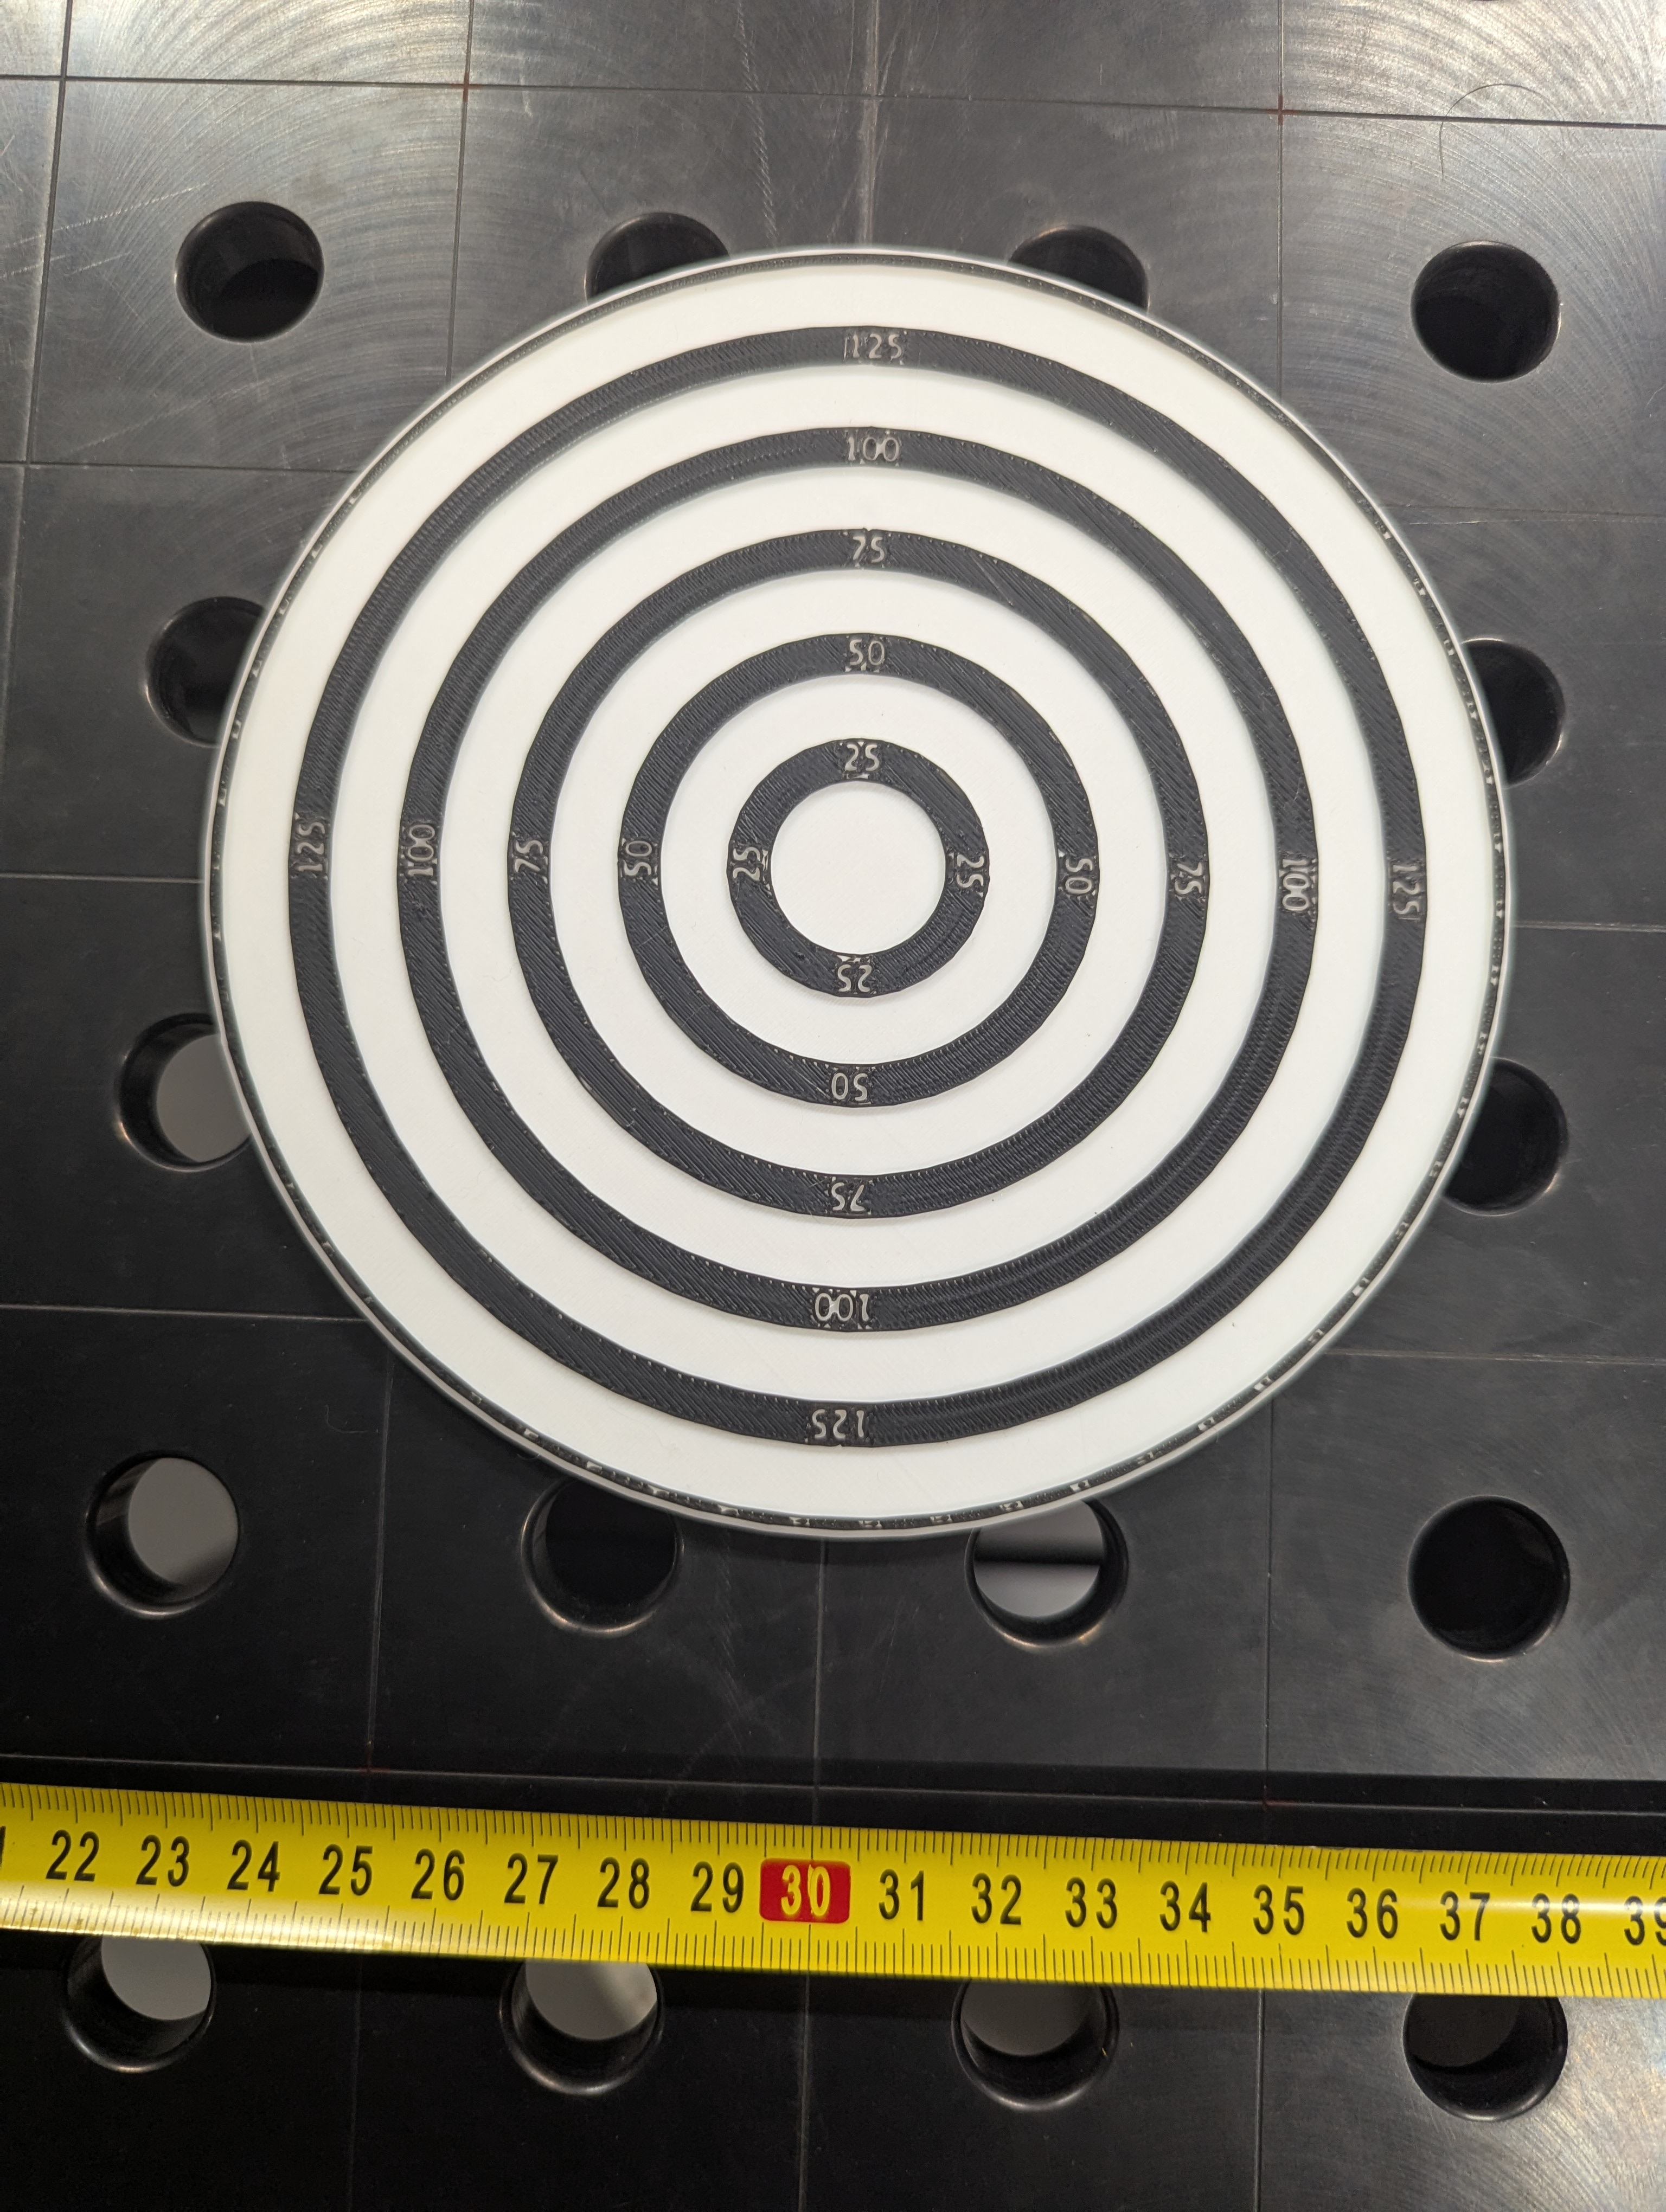
\includegraphics[width=\linewidth]{figures/precisionTest/shootingDiscX.jpg}
    \caption*{X direction of disc}
\end{minipage}
\hfill
\begin{minipage}{0.48\textwidth}
    \centering
    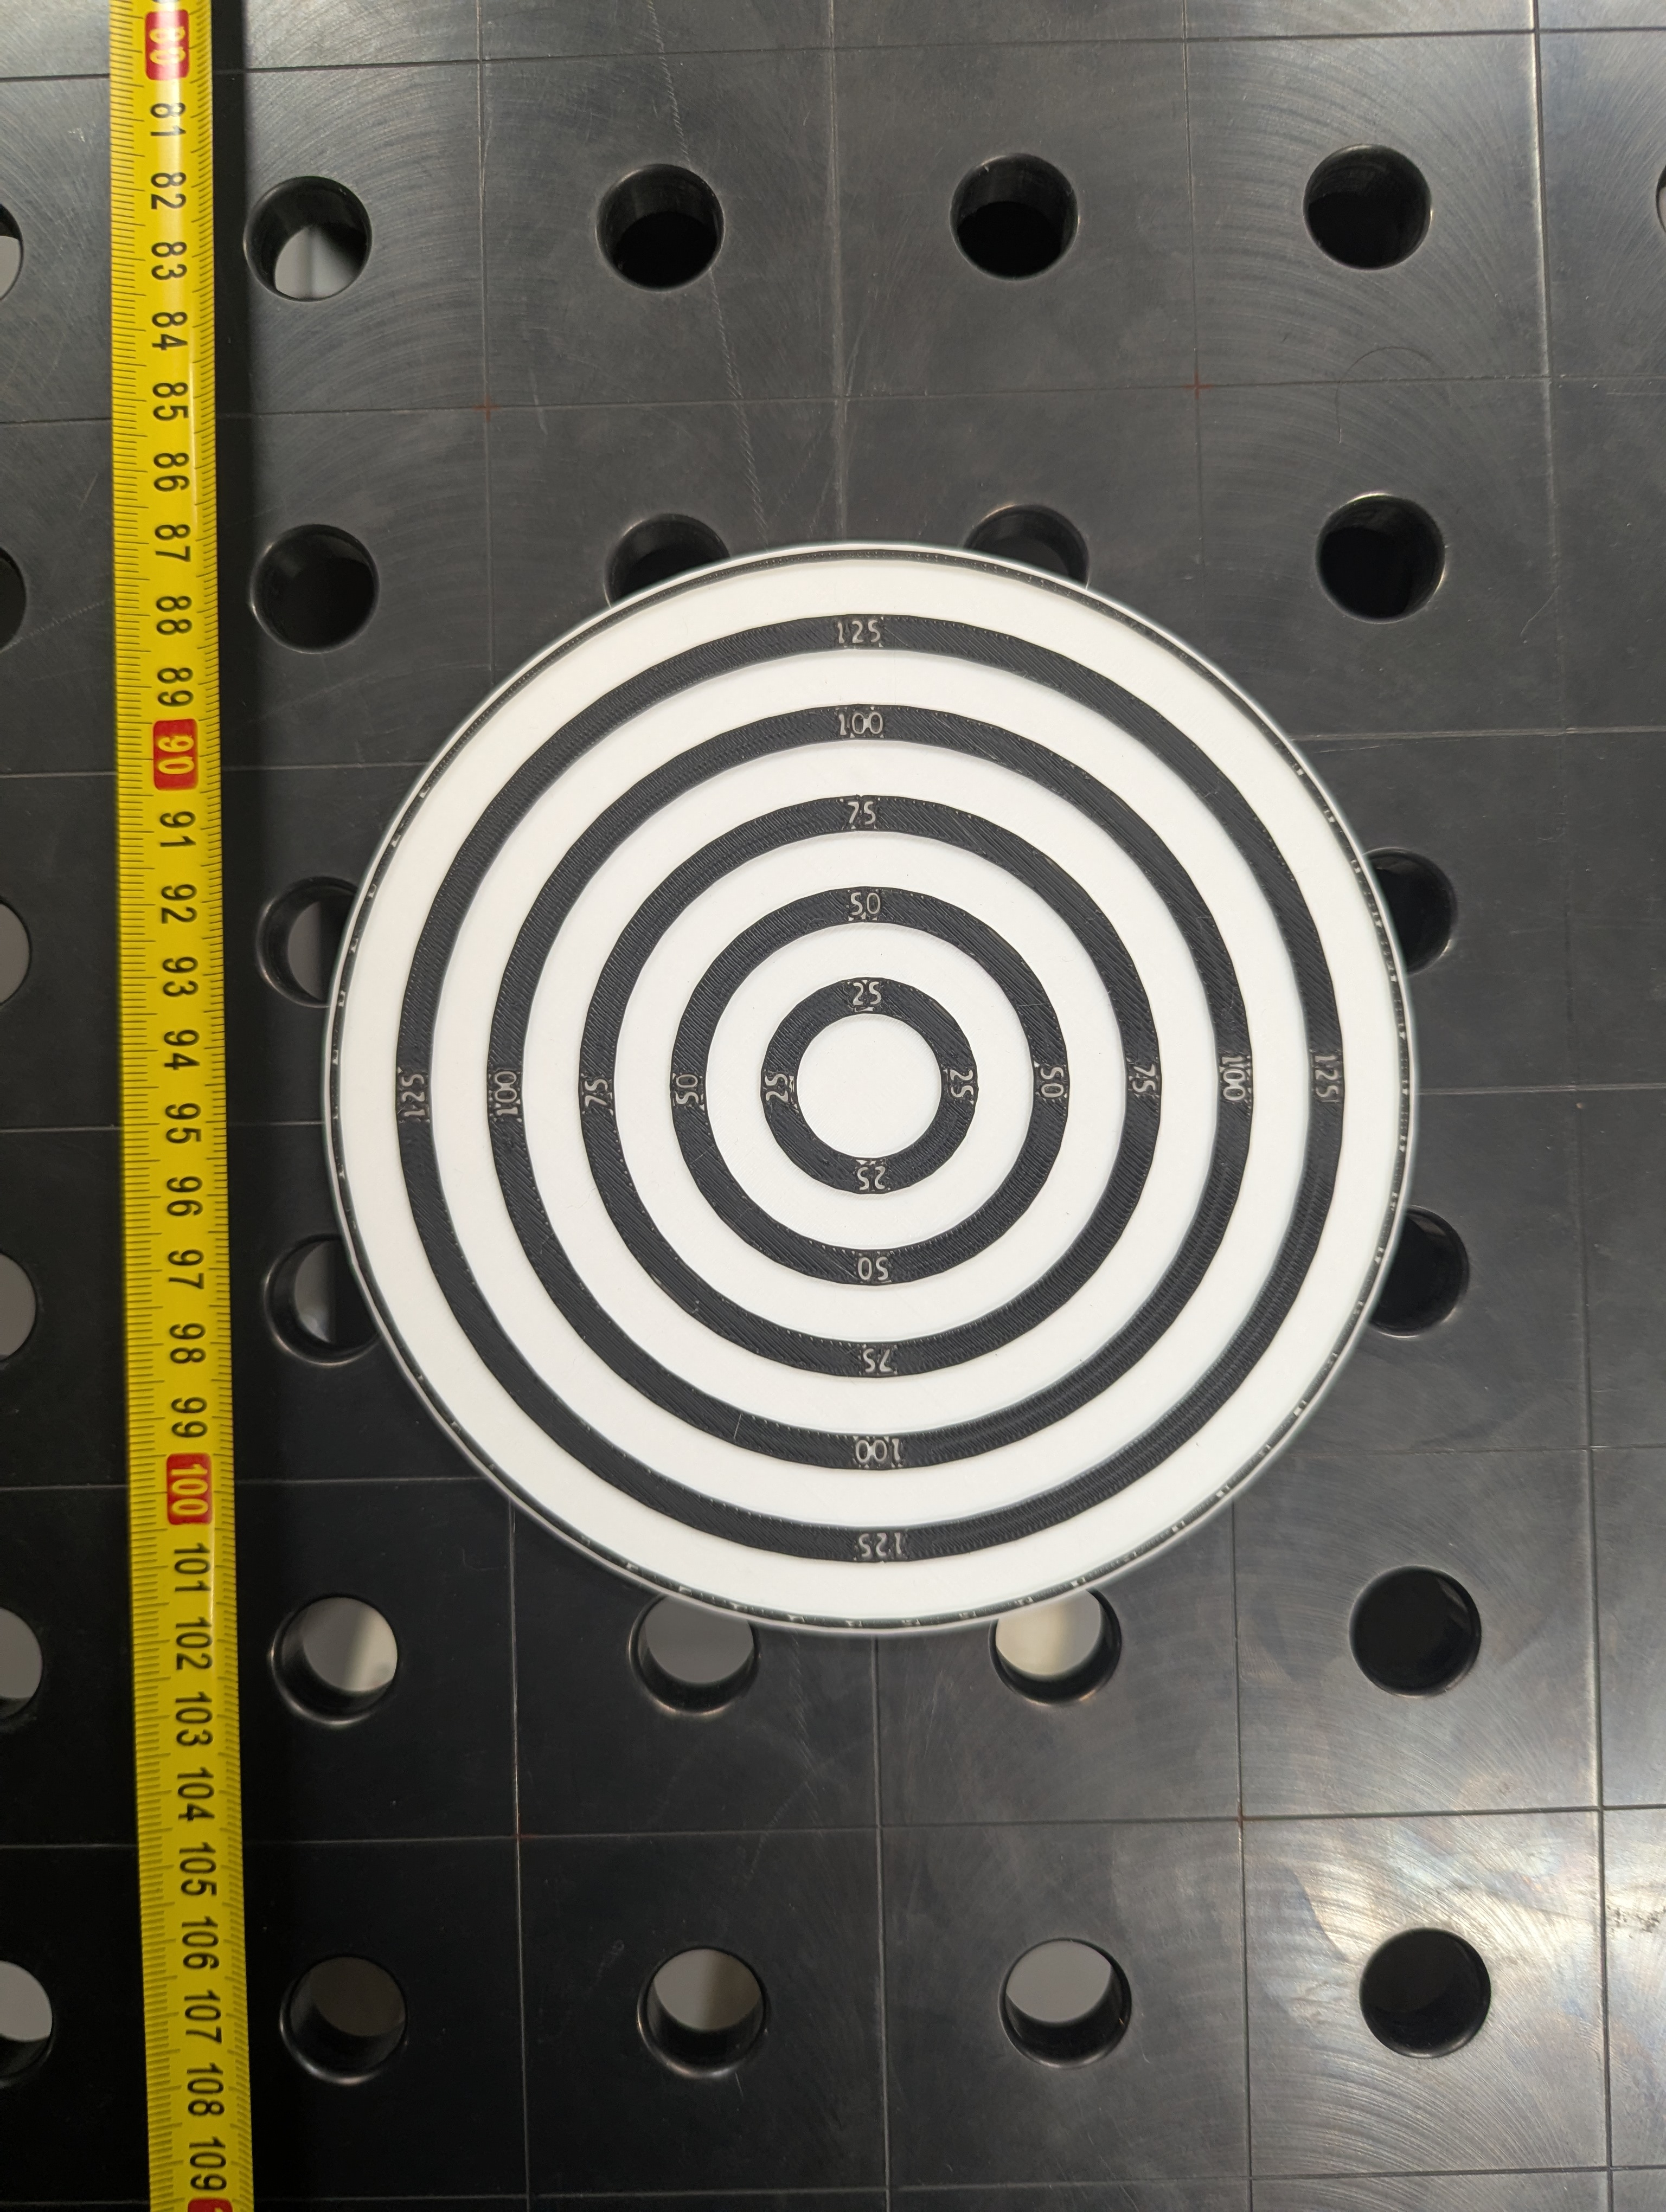
\includegraphics[width=\linewidth]{figures/precisionTest/shootingDiscY.jpg}
    \caption*{Y direction of disc}
\end{minipage}
\end{figure}
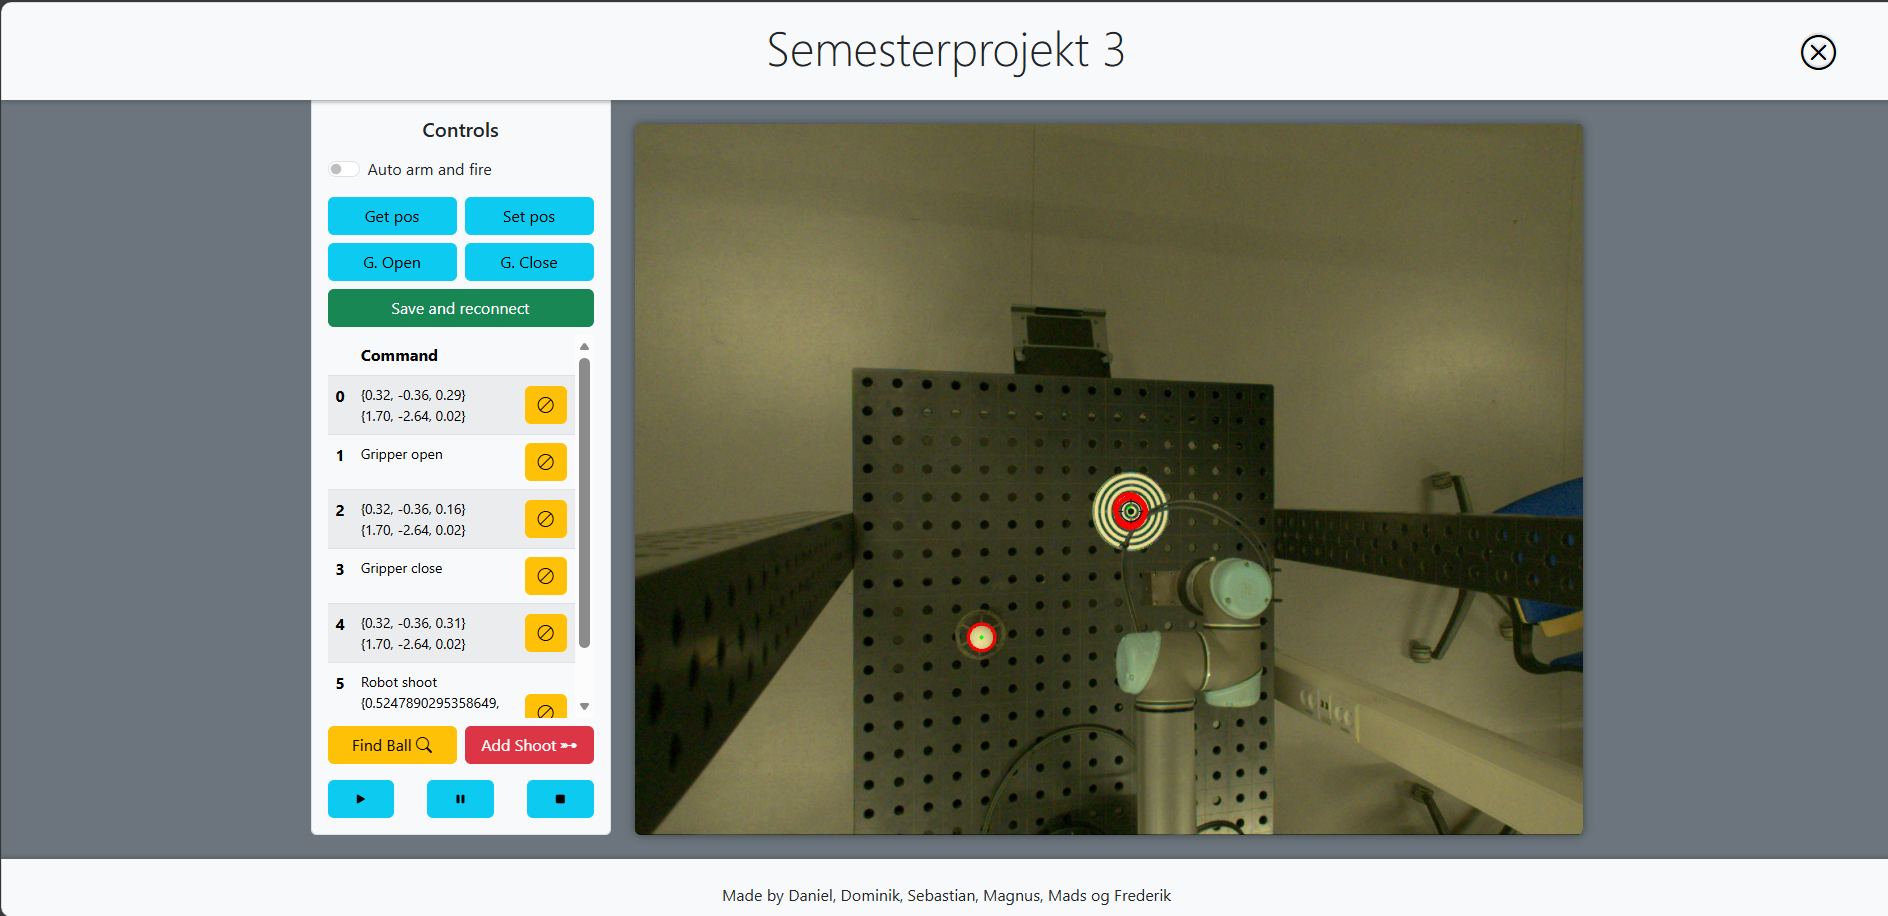
\includegraphics[width=100mm,center]{figures/precisionTest/screenShot.png}
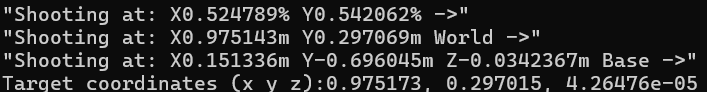
\includegraphics[width=190mm,center]{figures/precisionTest/testDetaljer.png}

As you can see, the x direction is a little off by 2,5cm in x+ direction, but the y direction is pretty much on point.

As it can be really hard to see how precise we hit, we have made a shooting disc. I will grade it with a inverted point system as to how good it hit it and if outside, i will grade it "out".

All the tests are videorecorded and can be found at "tests/servoJ\_VS\_speedJ precisionstest"

The disc is 150mm in diameter.

\subsubsection{servoJ precision}
\begin{tabular}{|c|c|}
\hline
test & result(mm) \\ \hline
1 & out \\ \hline
2 & out \\ \hline
3 & out \\ \hline
4 & 75 \\ \hline
5 & 50 \\ \hline
6 & 0 \\ \hline
7 & out \\ \hline
8 & out \\ \hline
9 & 50 \\ \hline
10 & 12.5 \\ \hline
11 & 50 \\ \hline
12 & 0 \\ \hline
13 & 50 \\ \hline

\end{tabular}

We hit the disc 8/13 times.\newline
The precision when it did hit the disc was about 36mm in radius which is much more precise than expected. 

\subsubsection{speedJ precision}

Here precision output has also been posted in corresponding folders

I will fail the test if we hit protective stop and call it PS which is also out.

\begin{tabular}{|c|c|}
\hline
test & result(mm) \\ \hline
1 & PS \\ \hline
2 & PS \\ \hline
3 & out \\ \hline
4 & 25 \\ \hline
5 & out \\ \hline
6 & out \\ \hline
7 & PS \\ \hline

\end{tabular}

We hit the disc 1/7 times.\newline
Also we hit protective stop 3/7 times.\newline
The precision when it did hit the disc was unusable. 

\subsection{Gripper response speed test} %kan godt være denne del skal flyttes til robotControl efter sektionen nu hedder evaluation og ikke tests
To ensure accuracy of our throw, it's important that we both release the ball while the robot is moving and at the correct position. This test will be focusing on the latter.
As out robot receives new positions to go to at a very quick speed (8ms), we need to ensure that the latency when sending a command to the gripper to when the gripper starts moving doesn't make our gripper release the ball at the wrong position.

The TCP communication works by us sending a command to the gripper and the gripper sending back an acknowledgement that it received the command before moving. By sending the command and then Immediately starting a timer that stops when we receive the ACK response meaning the gripper acknowledges the command and starts moving.

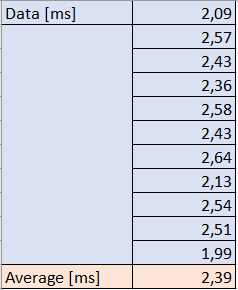
\includegraphics[width=50mm,center]{figures/GripData.PNG}
These are the 11 datapoints from said test. The average response time from the gripper to acknowledge the command is 2.39 ms which should result in no issues as to ensuring the ball is released at the correct time. If the ball is released exactly at the same time we receive the acknowledgement command, we can determine that the slight delay we get is irrelevant to the success of our throw.

However, what this test does not take into consideration is that just because we receive the confirmation that the gripper's fingers are moving, does not necessarily mean it immediately releases the ball at that exact time although it would seem like it from the naked eye. Ensuring this would require a much more extensive test. It is also possible that the gripper starts moving directly after it receives the command but before we receive the confirmation, reducing our delay time by perhaps half if it takes as much time to receive the confirmation as it did send the command.

\subsection{Final Product Testing}
To evaluate the final integrated product against the set goal, several tests were performed. The set goal was to hit the target 80  \% of all throws. The target counts as being hit, when the projectile lands within an orange 100 mm x 100 mm square box with a center point at the target position. 11 throws with varying target points were performed on this box and 3 out 11 throws were landed within the box. This gives a success rate of 27.27 \%. 

\


\newpage

\section{Discussion} 
\subsection{Kinematics}
The throw trajectory of the robot arm was calculated using cubic polynomials with specified joint angles and velocities at the start and end points. The calculated trajectories follow a linear movement in joint space, but a non-linear movement in cartesian space. Alternatively, the trajectory could follow a linear movement in cartesian space but a non-linear movement in joint space. Planning a linear movement in joint space makes it easier to find a trajectory to satisfy the joint space safety limits (table~\ref{tab:jointLimits}). However, planning a linear movement in cartesian space makes it easier to find a trajectory to satisfy the safety planes in cartesian space (table~\ref{tab:tcpLimits}). As we were given safety limitations in both the joint space and cartesian space, this made the trajectory planning particularly challenging. In the end we chose to use a linear movement in joint space. This was because the joint limits were the most restrictive compared to the cartesian limits, especially joint 5 which has only 40 degrees acceptable range. On top of that, trying to make a linear movement in cartesian space using the “cubicpolytraj” \cite{cubicPolyTraj} function resulted in the tcp making a curved movement between the specified points instead of connecting them in a straigth line. Therefore, it would be necessary to manually write a function if had chosen to make a linear movement in cartesian space. Another method to deal with the joint restrictions would be to lock the most problematic joint and do the kinematics without it. This would also require removing this joint from the Jacobian matrix when calculating the joint velocities \cite{kinematicsLecture10}. However, this approach was not chosen in the end, as not using all joints made it more difficult to find inverse kinematics solution for various transformation matrices. Finally, we chose cubic polynomials over quintic polynomials as it was not necessary to specify acceleration constraints, only velocity and position constraints. Alternatively, the cubic polynomials could be combined into a single trapezoidal velocity profile with the required joint velocities for the release point in the middle and 0 rad/s in the start and end for every joint. This is something that could be experimented in the future to further develop this project \cite{kinematicsLecture9}.

\subsection{Evaluation}
The tests for the final evaluation could be improved and expanded. First, instead of a square box, it would be better to use a round box. This is because for the square box the distance between the center and edge is larger in the corners than between the corners, while a round box has a constant radius all around. Additionally, instead of only testing 11 throws with random target coordinates leading to a single success rate, multiple targets could be tested systematically. This could be done by testing multiple points spread systematically over the table space with a fixed distance between them. The target box would be placed at each target point and multiple throws would be tested for each point. This would yield a success rate for each tested point across the table space. Using this data a 2D heat map of success rates across the table space could be created. From this data, a total average success rate over the whole tested space could be calculated. The same approach could also be taken for the accuracy test to create a heat map of the throw accuracy over the table space and to calculate the average accuracy over the whole tested space. 

\newpage

\section{Conclusion} 
\input{sections/Conclusion.tex}
\newpage

\nocite{*}
\printbibliography

\end{document}
